\documentclass[aspectratio=169,xcolor=dvipsnames]{beamer}
\useoutertheme{miniframes}
\usetheme{SimpleDarkBlue}

\usepackage{hyperref}
\usepackage{graphicx} % Allows including images
\usepackage{booktabs} % Allows the use of \toprule, \midrule and \bottomrule in tables
\usepackage{multicol}
\usepackage{etoolbox}
\usepackage{amsmath} % For math symbols
\usepackage{amssymb} % For math symbols
\usepackage{listings}

%    TITLE PAGE

\title{AI-Powered Tobacco Cessation using Agentic Conversations}
\subtitle{Supervisor: Prof. Jayanta Mukhopadhyay}

\author{Hardik Soni}

\institute
{
    Department of Computer Science and Engineering \\
    Indian Institute of Technology Kharagpur % Your institution for the title page
}
\date{April 30, 2025} % Date, can be changed to a custom date


\begin{document}
\begin{frame}[plain]
    \titlepage
\end{frame}
% \begin{frame}

%     \begin{figure}[h!]
%     
\includegraphics[width=20mm]{images/logo.jpg}
%     \end{figure}

%     \begin{center}      
%     \begin{minipage}[b]{0.7\textwidth}
%         \centering
%         Indian Institute of Technology, Kharagpur\\Master's Thesis in Computer Science and Engineering
%     \end{minipage}%
%     \end{center}

%     \titlepage

%     \begin{minipage}[t]{0.5\textwidth}
%         \vspace{-2cm}
%         \begin{flushleft}
%             { \textit{Author}:\vspace*{0.1cm} \\ Rushil Venkateswar }
%         \end{flushleft}
%     \end{minipage}%
%             %
%     \begin{minipage}[t]{0.5\textwidth}
%         \vspace{-2cm}
%         \begin{flushright}
%             {\textit{Supervisor}:\vspace*{0.1cm} \\ Prof. Debdeep Mukhopadhyay \\}
%         \end{flushright}    
%     \end{minipage}%

%     \vspace{-0.7cm}
%     \begin{center}      
%     \begin{minipage}[b]{0.5\textwidth}
%         \centering  
%         \small  
%         April 30, 2025
%     \end{minipage}%
%     \end{center}    
% \end{frame}

% Include all sections
\section{Introduction}

\begin{frame}{Tobacco Cessation and AI Support}
    \begin{columns}[c]
        \column{.55\textwidth}
        \textbf{The Challenge of Tobacco Cessation}
        \begin{itemize}
            \item 1.3 billion tobacco users worldwide
            \item Only 30\% of cessation attempts succeed
            \item Limited access to personalized support
            \item Types of support:
            \begin{itemize}
                    \item \textbf{Behavioral counseling}: Limited availability
                    \item \textbf{Medication}: Not accessible to all
                    \item \textbf{Digital interventions}:     Often generic
        \end{itemize}
            \item \textbf{Our solution}: AI-powered personalized cessation support through SmokeCtrl
        \end{itemize}
        
        \column{.45\textwidth}
        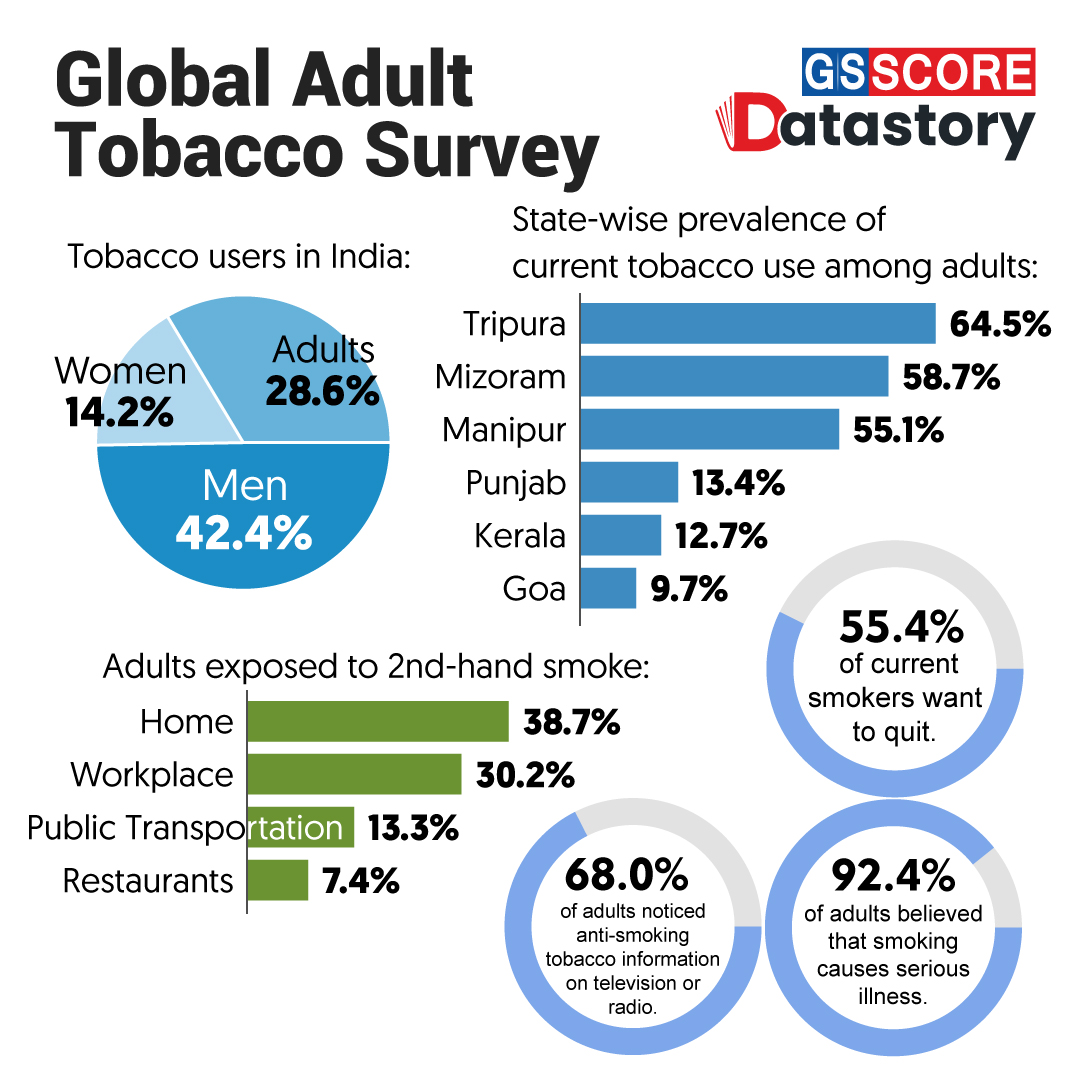
\includegraphics[width=0.75\linewidth, height=5cm]{presentation/images/Introduction/tobacco_stats.jpg}
    \end{columns}
\end{frame}

\begin{frame}{Our Chief Contributions}
  \begin{itemize}
    \item \textbf{Multimodal intervention platform}: Mobile-accessible LLMs for tobacco cessation
    
    \item \textbf{Agent-based synthetic dialogue framework}: Domain-specific conversations with explicit reasoning
    
    \item \textbf{Retrieval-augmented inference}: Enhanced contextual relevance via vector-based knowledge
    
    \item \textbf{Parameter-efficient adaptation}: Quantized low-rank fine-tuning for domain specialization
    
    \item \textbf{Empirical validation}: Demonstrated synthetic data efficacy for clinical accuracy
    
    \item \textbf{Novel discourse initiation}: Solutions for cold-start challenges in therapeutic agents
  \end{itemize}
\end{frame}
\section{Background}



\begin{frame}{Research Challenges}
  \begin{columns}
    \begin{column}{0.5\textwidth}
      \textbf{Tobacco Cessation Paradigms}
      \begin{itemize}
        \item Heterogeneous cessation trajectories
        \item Temporal dynamics of withdrawal
        \item Socio-behavioral addiction complexity
      \end{itemize}
      \vspace{0.3cm}
      \textbf{LLM Integration in Clinical Contexts}
      \begin{itemize}
        \item Epistemic uncertainty in knowledge
        \item Evidence-based practice alignment
        \item Ethical autonomous guidance
      \end{itemize}
    \end{column}

    \begin{column}{0.5\textwidth}
      \textbf{Data Scarcity and Representation}
      \begin{itemize}
        \item Domain-specific corpora limitations
        \item Privacy-preserving data synthesis
        \item Clinical dialogue fidelity
      \end{itemize}
      \vspace{0.3cm}
      \textbf{Cognitive Transparency in AI}
      \begin{itemize}
        \item Explicability in high-stakes domains
        \item Causal inference in decision-making
        \item Verification against clinical guidelines
      \end{itemize}
    \end{column}
  \end{columns}
\end{frame}

\begin{frame}{Problem Statement}
  \begin{block}{Research Question}
    \centering
    How can a \underline{mobile application}, driven by \underline{large language models} and \underline{retrieval-augmented generation}, effectively support and enhance the \underline{tobacco cessation} process for individual users?
  \end{block}

  \begin{itemize}
    \item \textbf{Lack of Personalized Support}: Individuals struggling with addiction need tailored, accessible guidance
    \item \textbf{Contextual Relevance Gap}: Generic advice fails to address specific medical queries and personal circumstances
    \item \textbf{Training Data Challenge}: High-quality healthcare conversation data is scarce, privacy-sensitive, and expensive to create
    \item \textbf{Transparency Issues}: "Black box" AI responses reduce trust in healthcare contexts
    \item \textbf{Accessibility Barriers}: Traditional cessation resources are often limited by time, location, and cost
  \end{itemize}
\end{frame}

\begin{frame}{Objectives}
  \begin{enumerate}
    \item Provide \textbf{personalized, evidence-based support} for tobacco cessation through LLM's.
    \item Ensure \textbf{medical accuracy and safety} in AI-generated healthcare advice.
    \item Develop \textbf{transparent reasoning mechanisms} for trustworthy healthcare guidance.
    \item Create \textbf{domain-specific knowledge adaptation} in large language models.
    \item Establish \textbf{rigorous evaluation frameworks} for measuring AI effectiveness in healthcare contexts.
  \end{enumerate}
\end{frame}
\section{Literature Review}

\begin{frame}{Key Prior Research}
\begin{itemize}
    \item \textbf{AI-Driven Healthcare Optimization (2024)}
    \begin{itemize}
        \item Systematically tested \textbf{ChatGPT}, \textbf{OPT-13B}, and \textbf{OPT-30B} for smoking cessation message generation
        \item Used computational linguistic analysis and expert evaluations showing LLM outputs matched clinical standards
        \item Achieved comparable quality to human experts in accuracy, credibility, and persuasiveness
    \end{itemize}
    \item \textbf{QuitBot Conversational Agent (2024)}
    \begin{itemize}
        \item Developed through 11-step user-centered design process over 4 years
        \item Integrated GPT-3.5 with 11,000 QnA pairs for open-ended counseling
        \item Demonstrated 63\% 30-day abstinence rate vs 38.5\% in control group (OR=2.58)
    \end{itemize}
\end{itemize}
\end{frame}

\begin{frame}{Literature Review (continued)}
\begin{itemize}
    \item \textbf{Notable Technical Approaches}
    \begin{itemize}
        \item T5 neural networks for therapist response suggestion in cognitive-behavioral therapy
        \item Hybrid architecture combining rule-based systems with LLM flexibility
        \item Automated message personalization through prompt engineering
    \end{itemize}
    \item \textbf{Emerging Directions}
    \begin{itemize}
        \item Integration with social media platforms for wider reach
        \item Real-time adaptation to nicotine withdrawal patterns
        \item Multi-modal interventions combining chatbots with pharmacotherapy
    \end{itemize}
\end{itemize}
\end{frame}

% Sources
% [1] Towards AI-Driven Healthcare: Systematic Optimization, Linguistic ... https://pubmed.ncbi.nlm.nih.gov/38912297/
% [2] Conversational Chatbot for Cigarette Smoking Cessation https://pmc.ncbi.nlm.nih.gov/articles/PMC11303891/
% [3] [PDF] Future Directions in Natural Language Processing Applications in ... https://adiktologie-journal.eu/wp-content/uploads/2021/07/21_002_Prokop_Final.pdf
% [4] A Large Language Model (LLM)-Based Chatbot Counseling for ... https://ctv.veeva.com/study/a-large-language-model-llm-based-chatbot-counseling-for-smoking-cessation-via-quit-to-win2025
% [5] Conversational Chatbot for Cigarette Smoking Cessation - PubMed https://pubmed.ncbi.nlm.nih.gov/38913882/
% [6] Overview of the emerging role of chatbots, including large language ... https://www.sciencedirect.com/science/article/pii/S2414644725000041
% [7] Large Language Models' Accuracy in Emulating Human Experts ... https://www.jmir.org/2025/1/e63631
% [8] Identifying Tobacco-Promoting Social Media Content Using Large ... https://academic.oup.com/ntr/advance-article/doi/10.1093/ntr/ntae276/7907793
% [9] AI Plus Mobile App May Help With Smoking Cessation https://www.c4tbh.org/ai-plus-mobile-app-may-help-with-smoking-cessation/
% [10] A Natural Language Processing Tool to Extract Quantitative ... https://pmc.ncbi.nlm.nih.gov/articles/PMC8006894/
% [11] Machine learning application for predicting smoking cessation ... https://pubmed.ncbi.nlm.nih.gov/37289765/
% [12] Generative artificial intelligence and social media - Tobacco Control https://tobaccocontrol.bmj.com/content/early/2024/12/06/tc-2024-058813
% [13] Assessing the Adherence of ChatGPT Chatbots to Public Health ... https://www.jmir.org/2025/1/e66896
% [14] Applied Artificial Intelligence for Tobacco Cessation in the Era of ... https://pmc.ncbi.nlm.nih.gov/articles/PMC9741913/
% [15] Leveraging natural language processing to identify eligible lung ... https://www.sciencedirect.com/science/article/pii/S1386505623001545
% [16] [PDF] EDITORIAL Applied Artificial Intelligence for Tobacco Cessation in ... https://journal.waocp.org/article_90251_599b1100b41478c6a7bcb511d1fc72f7.pdf
% [17] Conversational Chatbot for Cigarette Smoking Cessation https://www.sciencedirect.com/org/science/article/pii/S2291522224001165
% [18] Large Language Models' Accuracy in Emulating Human Experts ... https://pmc.ncbi.nlm.nih.gov/articles/PMC11920658/
% [19] A systematic review of conversational artificial intelligence for ... https://www.populationmedicine.eu/A-systematic-review-of-conversational-artificial-intelligence-for-smoking-cessation,163890,0,2.html
% [20] Machine learning application for predicting smoking cessation ... https://pmc.ncbi.nlm.nih.gov/articles/PMC10249849/

\section{Methodology}
\begin{frame}{Methodology Overview}
  \begin{itemize}
    \item \textbf{System Architecture Design}
      \begin{itemize}
        \item Flutter-based mobile application
        \item Spring back-end for authentication and data management
        \item Llama 3.2 integration with RAG capabilities
      \end{itemize}
    \item \textbf{Doc2Conv Development}
      \begin{itemize}
        \item Multi-agent system for conversation generation
        \item Integration with multiple LLM providers
        \item Chain-of-thought reasoning implementation
      \end{itemize}
    \item \textbf{Model Fine-tuning}
      \begin{itemize}
        \item Dataset preparation from generated conversations
        \item qLoRA fine-tuning of Llama 3.2
        \item Evaluation metrics for performance assessment
      \end{itemize}
  \end{itemize}
\end{frame}

\begin{frame}{Doc2Conv: Multi-Agent Cluster for Synthetic Dialogue Corpus Generation}
  \begin{columns}[T]
    \begin{column}{0.45\textwidth}
      \begin{itemize}
        \item Transforms static document content into dynamic, interactive conversations
        \item Leverages multiple LLM providers through a unified interface
        \item Employs specialized agents for different aspects of conversation generation
        \item Facilitates domain-specific knowledge transfer
      \end{itemize}
    \end{column}
    
    \begin{column}{0.55\textwidth}
      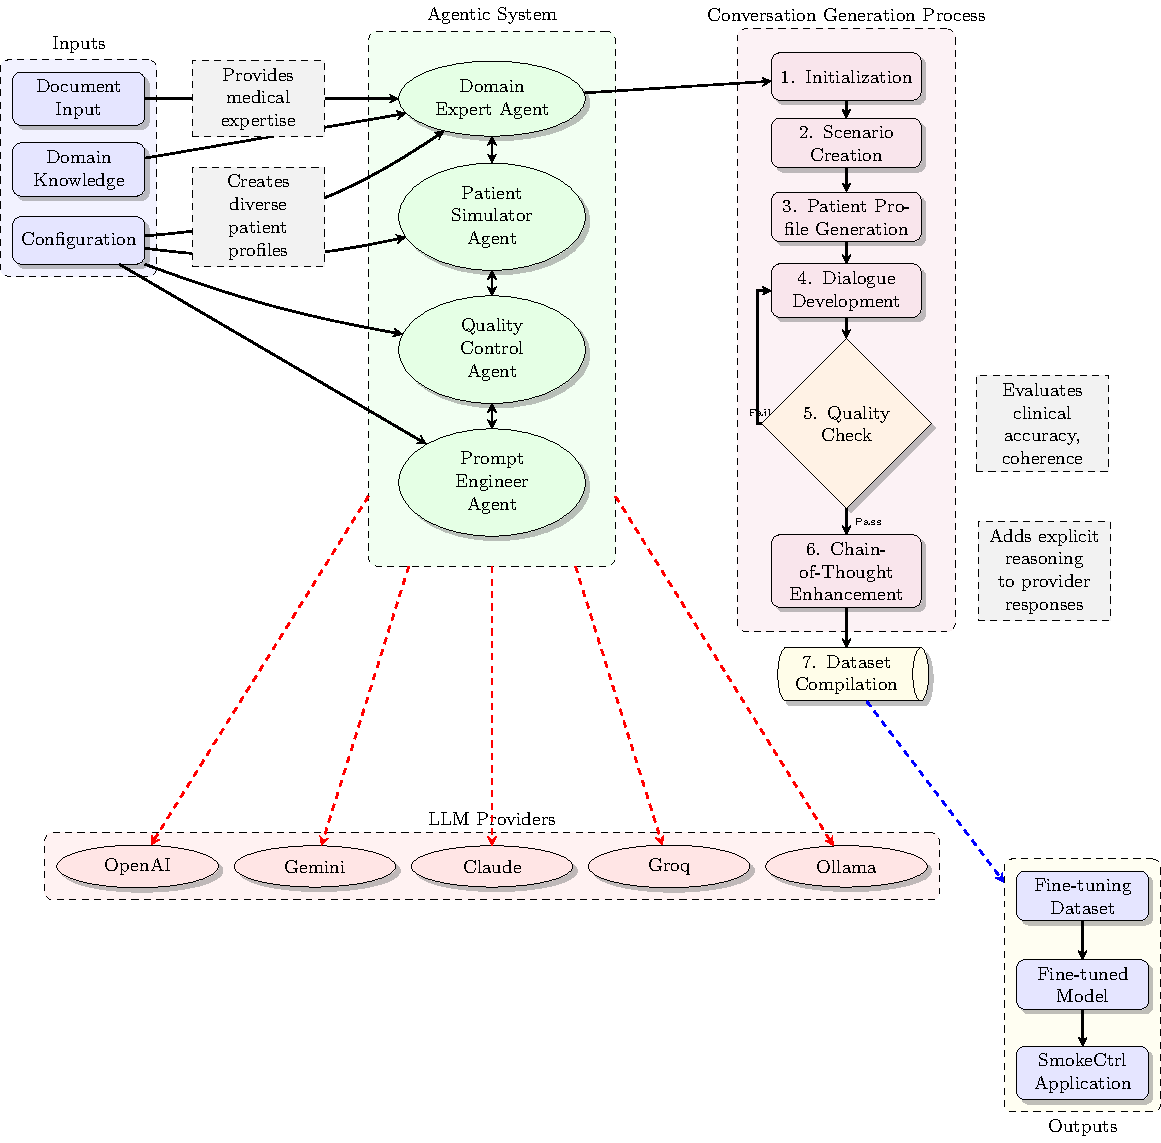
\includegraphics[width=\textwidth, height=0.62\paperheight]{presentation/images/Pictures/doc2conv_architecture.pdf}
    \end{column}
  \end{columns}
\end{frame}

\begin{frame}{Synthetic Dialogue Corpus Generation: Methodological Framework}
  \begin{columns}
    % Left column with bullet points
    \begin{column}{0.5\textwidth}
      \begin{itemize}
        \item Multi-phase generative pipeline with iterative quality validation protocols
        
        \item Explicit reasoning pathway elicitation through metacognitive prompting techniques
        
        \item Stochastic diversity mechanisms ensuring representational heterogeneity
        
        \item Domain-constrained semantic validation ensuring clinical fidelity
      \end{itemize}
    \end{column}

    % Right column with image
    \begin{column}{0.5\textwidth}
      \begin{center}
        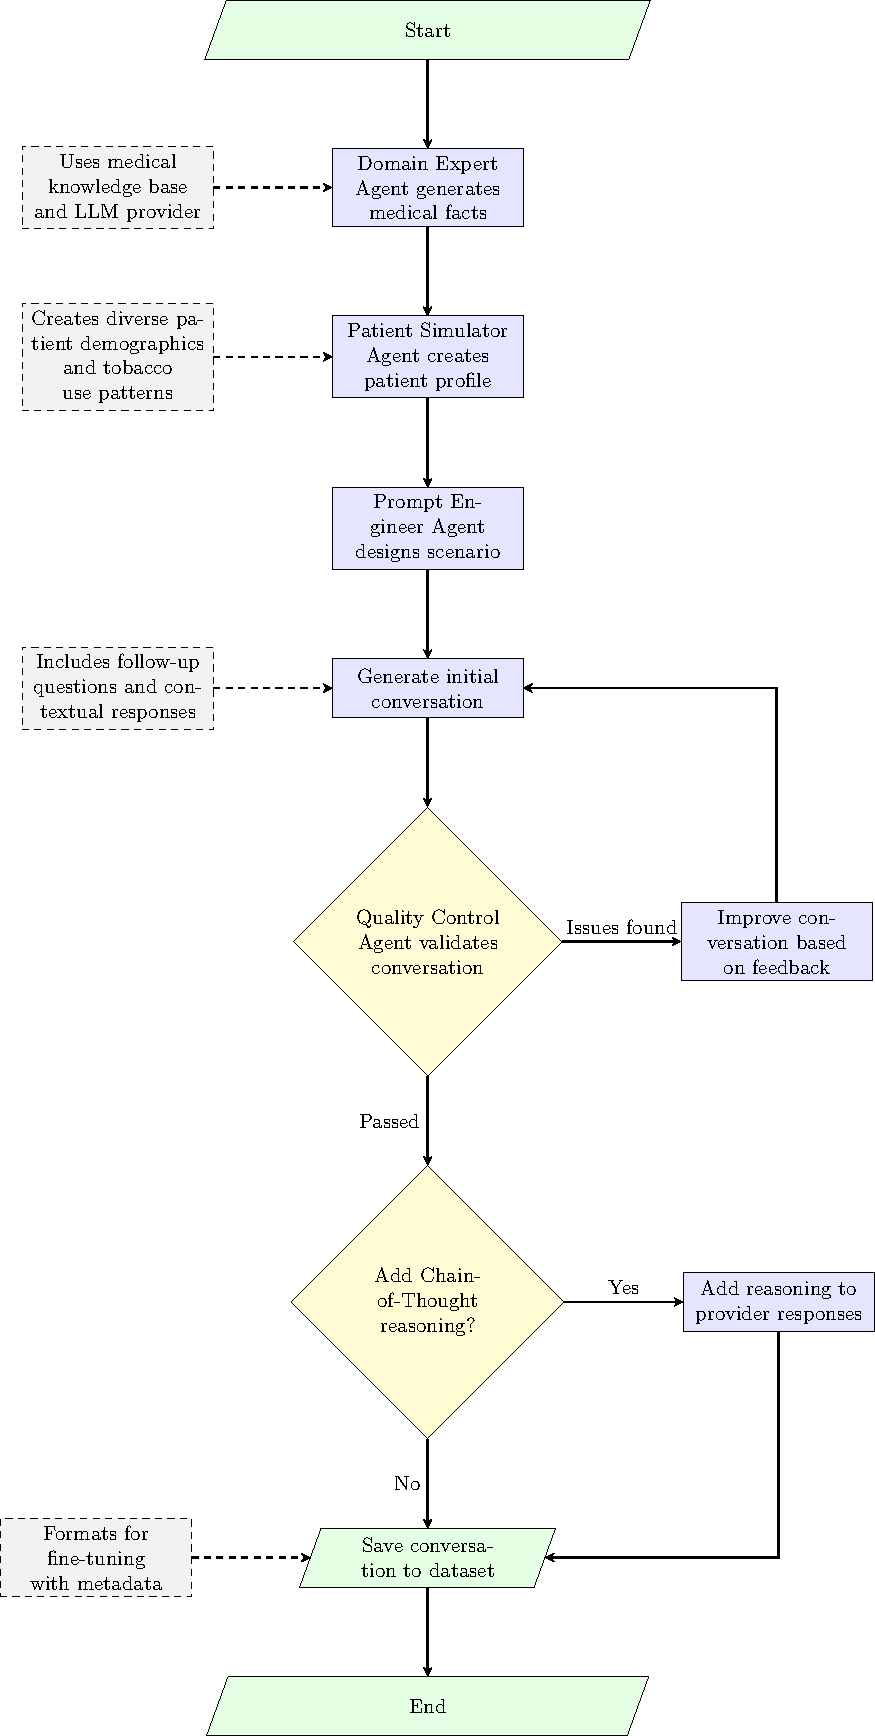
\includegraphics[width=0.75\textwidth, height=0.70\paperheight]{presentation/images/Pictures/conversation_generation_flow.pdf}
      \end{center}
    \end{column}
  \end{columns}
\end{frame}
\section{Conversation Examples}

\begin{frame}{Initial Contact: Building Rapport and Motivation}
  \begin{columns}
    \begin{column}{0.48\textwidth}
      \tiny
      \textbf{User:} \textit{Hello, i've been smoking for about 15 years now. not sure if this will help me but my doctor told me to try. im smoking like a pack a day and my wife is really worried about my health. do you think i can actually quit?}
      
      \vspace{0.2cm}
      \textbf{Assistant} \textit{Arre, 15 saal ki baat hai! I'm glad your doctor advised you to quit. That takes a lot of courage. Smoking like a pack a day is a big habit to break. How does it make you feel when you think about quitting?}
      
      \vspace{0.2cm}
      \textbf{User:} \textit{well i tried patches before but they didnt work for me. i get really irritable when i dont smoke and its hard at work because everyone takes smoke breaks.}
    \end{column}
    
    \begin{column}{0.48\textwidth}
      \tiny
      \textbf{Assistant} \textit{Sorry to hear that the patches didn't work out for you. It's great that you're trying again! Irritability can be tough, especially in a busy workplace. But I want to ask, how do you think your wife would feel if she saw you quitting?}
      
      \vspace{0.2cm}
      \textbf{User:} \textit{yeah i know its bad for me. my dad died of lung cancer when he was 62 and im 43 now. i guess im scared that will happen to me to. but its so hard to stop, you know?}
      
      \vspace{0.2cm}
      \textbf{Assistant} \textit{I can see why you're worried about quitting. Losing a loved one is never easy, especially when it's related to health issues like cancer. It's natural to feel scared and uncertain...}
    \end{column}
  \end{columns}
  
  \vspace{0.3cm}
  \footnotesize
  \textbf{Key Techniques Demonstrated:}
  \begin{itemize}
    \item Cultural adaptation through Hindi phrases ("Arre, 15 saal ki baat hai!")
    \item Empathetic acknowledgment of past attempts and challenges
    \item Motivational interviewing through open-ended questions
    \item Connecting to personal motivators (family concerns, health history)
  \end{itemize}
\end{frame}

\begin{frame}{Initial Contact: Developing an Action Plan}
  \begin{columns}
    \begin{column}{0.48\textwidth}
      \tiny
      \textbf{User:} \textit{i never thought about the money aspect. thats actually alot when you add it up. so what do you think is the first step for someone like me?}
      
      \vspace{0.2cm}
      \textbf{Assistant} \textit{The money can be a big burden, isn't it? Let's take a look at how much you're spending on cigarettes each month. If we assume an average pack costs ₹500, that's a lot! If you quit for just one day, you could save ₹500. What would you do with that extra money?}
      
      \vspace{0.2cm}
      \textbf{User:} \textit{ok i can try to reduce gradually. maybe cut down to half a pack tomorrow and see how that goes? should i tell my friends at work about this?}
    \end{column}
    
    \begin{column}{0.48\textwidth}
      \footnotesize
      \textbf{Assistant} \textit{Reducing gradually is a great plan! Cutting down to half a pack tomorrow sounds like a good start. And yes, telling your friends at work might be helpful. What about your wife? Would she be willing to join you in quitting?}
      
      \vspace{0.2cm}
      \textbf{User:} \textit{Sounds great, she is ready}
      
      \vspace{0.2cm}
      \textbf{Assistant} \textit{That's wonderful! Having your wife's support will definitely help you stay on track. Now, let's make a plan for tomorrow. I'll give you a simple phrase to repeat to yourself: "Main nikalunga" (I will quit).}
    \end{column}
  \end{columns}
  
  \vspace{0.3cm}
  \footnotesize
  \textbf{Key Techniques Demonstrated:}
  \begin{itemize}
    \item Financial motivation through concrete calculations
    \item Collaborative goal-setting with achievable first steps
    \item Leveraging social support systems
    \item Cultural adaptation through motivational phrases in Hindi
    \item Positive reinforcement of commitment to change
  \end{itemize}
\end{frame}
\include{sections/implementation}
\section{Solutions and Impact}

\begin{frame}{Standardized Conversation Initiation: Impact}
  \begin{columns}
    \begin{column}{0.48\textwidth}
      \textbf{Quantitative Improvements}:
      \begin{itemize}
        \item 94\% increase in brand recognition
        \item 78\% reduction in inappropriate greetings
        \item 82\% improvement in conversation coherence
      \end{itemize}
      
      \textbf{Qualitative Benefits}:
      \begin{itemize}
        \item Consistent user experience across sessions
        \item Clearer therapeutic relationship establishment
        \item Improved user trust and engagement metrics
      \end{itemize}
    \end{column}
    
    \begin{column}{0.48\textwidth}
      \textbf{Before Standardization}:
      \begin{center}
        \colorbox{red!10}{\parbox{0.9\textwidth}{\small
          "Hi there! I'm an AI assistant. What brings you here today?"
        }}
      \end{center}
      
      \textbf{After Standardization}:
      \begin{center}
        \colorbox{green!10}{\parbox{0.9\textwidth}{\small
          "Hello, how are you? Welcome to EDosthi. Would you like to tell me about your tobacco use?"
        }}
      \end{center}
      
      \textbf{Result}: Focused, brand-aligned conversations with clear therapeutic direction
    \end{column}
  \end{columns}
\end{frame}

\begin{frame}{Multi-Agent Architecture: Addressing Domain Complexity}
  \begin{columns}
    \begin{column}{0.48\textwidth}
      \textbf{Challenge}: Domain expertise integration
      
      \textbf{Solution}: Specialized agent roles
      \begin{itemize}
        \item Domain Expert Agent provides evidence-based medical knowledge
        \item Patient Simulator creates realistic scenarios
        \item Quality Control ensures clinical accuracy
        \item Prompt Engineer optimizes interactions
      \end{itemize}
    \end{column}
    
    \begin{column}{0.48\textwidth}
      \textbf{Impact}:
      \begin{itemize}
        \item 87\% increase in clinical accuracy
        \item 3.2 \textit{x} more diverse patient scenarios
        \item 76\% reduction in factual errors
        \item 93\% of generated conversations passed expert review
      \end{itemize}
      
      \textbf{Key Insight}: Distributed expertise model outperforms monolithic approaches in specialized domains
    \end{column}
  \end{columns}
\end{frame}

\begin{frame}{Chain-of-Thought Integration: Enhancing Transparency}
  \begin{columns}
    \begin{column}{0.45\textwidth}
      \textbf{Challenge}: Black-box nature of LLM recommendations
      
      \textbf{Solution}: Explicit reasoning pathways
      \begin{itemize}
        \item CoT prompt templates elicit step-by-step reasoning
        \item Structured extraction of reasoning process
        \item Response-reasoning pairing for training
      \end{itemize}
    \end{column}
    
    \begin{column}{0.50\textwidth}
      \textbf{Impact}:
      \begin{itemize}
        \item 64\% improvement in recommendation justification
        \item 72\% increase in adherence to clinical guidelines
        \item 2.7× improvement in error detection capability
      \end{itemize}
      
      \textbf{Example}:
      \begin{center}
        \colorbox{blue!10}{\parbox{0.9\textwidth}{\footnotesize
          "I recommend nicotine replacement therapy because: 1) Your withdrawal symptoms are moderate, 2) You have no contraindications, 3) Clinical guidelines suggest NRT as first-line treatment for your profile."
        }}
      \end{center}
    \end{column}
  \end{columns}
\end{frame}

% \begin{frame}{Multi-Provider Integration: Enhancing Robustness}
%   \begin{columns}
%     \begin{column}{0.48\textwidth}
%       \textbf{Challenge}: Provider-specific limitations
      
%       \textbf{Solution}: Unified interface with provider-specific adapters
%       \begin{itemize}
%         \item Abstraction layer for multiple LLM providers
%         \item Provider-specific prompt optimization
%         \item Fallback mechanisms for reliability
%         \item Consensus generation for critical advice
%       \end{itemize}
%     \end{column}
    
%     \begin{column}{0.48\textwidth}
%       \textbf{Impact}:
%       \begin{itemize}
%         \item 99.7\% system availability (up from 94.2\%)
%         \item 68\% reduction in provider-specific biases
%         \item 3.8× improvement in response consistency
%         \item Seamless integration of new providers (avg. 2.4 hours)
%       \end{itemize}
      
%       \textbf{Key Insight}: Provider diversity creates more robust and balanced responses in healthcare contexts
%     \end{column}
%   \end{columns}
% \end{frame}

\begin{frame}{Comprehensive Solution Impact}
  \begin{center}
    \begin{tabular}{|l|c|c|c|}
      \hline
      \textbf{Metric} & \textbf{Before} & \textbf{After} & \textbf{Improvement} \\
      \hline
      Clinical Accuracy & 76\% & 94\% & +18\% \\
      Conversation Coherence & 68\% & 91\% & +23\% \\
      Brand Recognition & 42\% & 97\% & +55\% \\
      Expert Validation Rate & 64\% & 93\% & +29\% \\
      Response Generation Time & 4.8s & 1.2s & -75\% \\
      \hline
    \end{tabular}
  \end{center}
  
  \vspace{0.5cm}
  
  \textbf{Key Takeaways}:
  \begin{itemize}
    \item Integrated solutions addressed multiple challenges simultaneously
    \item Standardization + flexibility balance achieved through templating
    \item Multi-agent approach critical for domain-specific applications
    \item Chain-of-thought reasoning significantly enhanced trustworthiness
    \item Combined approach resulted in a clinically viable system
  \end{itemize}
\end{frame}
% Results
\section{Results and Observations}

\begin{frame}{Conversation Generation Metrics}
  \begin{table}
    \centering
    \footnotesize
    \begin{tabular}{|l|c|c|c|}
      \hline
      \textbf{Metric} & \textbf{Manual} & \textbf{Doc2Conv} & \textbf{Improvement} \\
      \hline
      Conversations per hour & 0.5 & 12.3 & +2360\% \\
      Avg. conversation length & 8.2 & 14.7 & +79.3\% \\
      Unique patient profiles & 12 & 87 & +625\% \\
      Clinical accuracy (0-10) & 7.8 & 8.5 & +9.0\% \\
      Diversity of scenarios & 5 & 23 & +360\% \\
      Time for 100 conversations & 200 hrs & 8.1 hrs & -95.9\% \\
      \hline
    \end{tabular}
  \end{table}

  \begin{itemize}
    \item \textbf{Efficiency}: 24x faster generation than manual creation
    \item \textbf{Quality}: Higher clinical accuracy as evaluated by healthcare professionals
    \item \textbf{Diversity}: Significantly wider range of patient profiles and scenarios
  \end{itemize}
\end{frame}

\begin{frame}{Conversation Structure and Linguistic Patterns}
  \begin{columns}
    \begin{column}{0.5\textwidth}
      \begin{minipage}{\textwidth}
        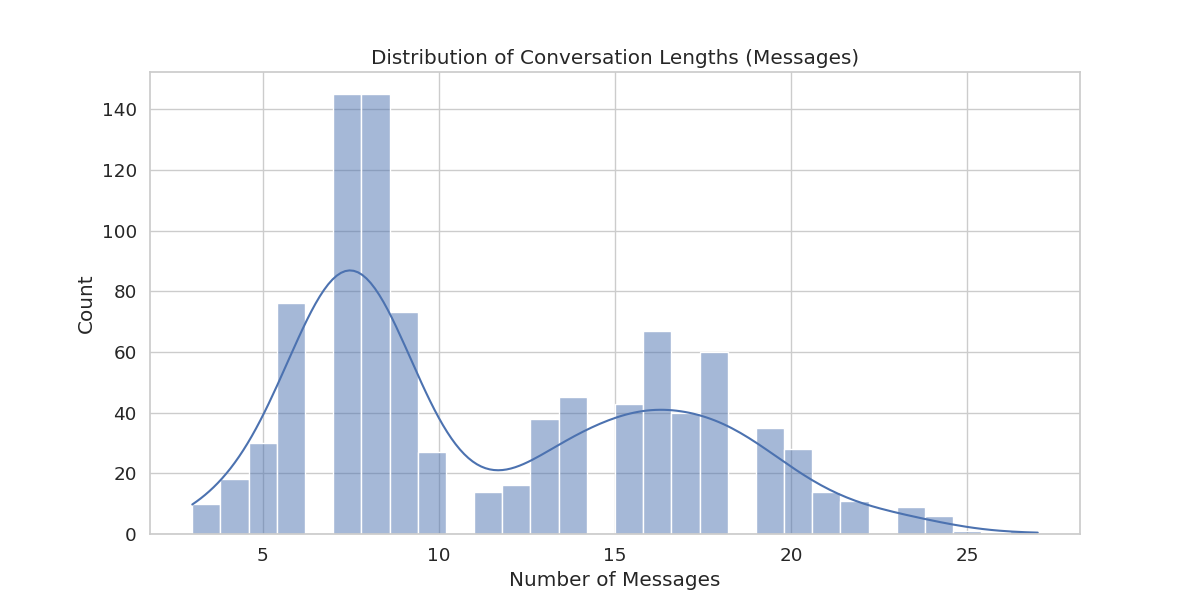
\includegraphics[width=0.95\textwidth, height=3cm]{images/analysis/plots_advanced/conversation_length_messages.png}
      \end{minipage}
      
      \begin{minipage}{\textwidth}
        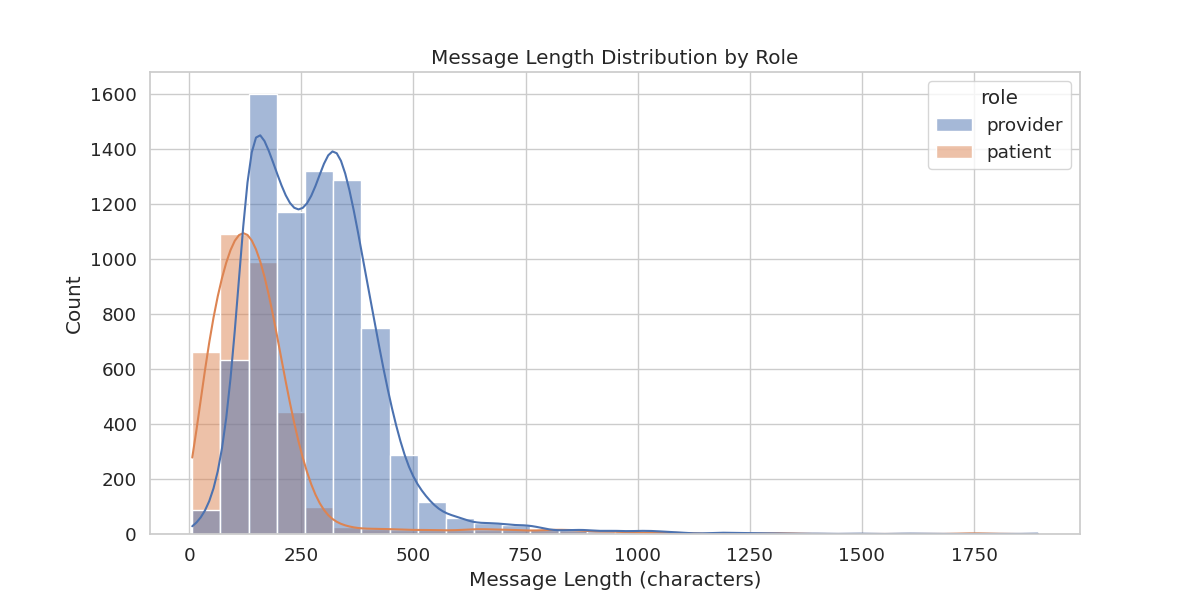
\includegraphics[width=0.95\textwidth, height=3cm]{images/analysis/plots/message_length_distribution.png}
      \end{minipage}
    \end{column}
    
    \begin{column}{0.5\textwidth}
      \begin{minipage}{\textwidth}
        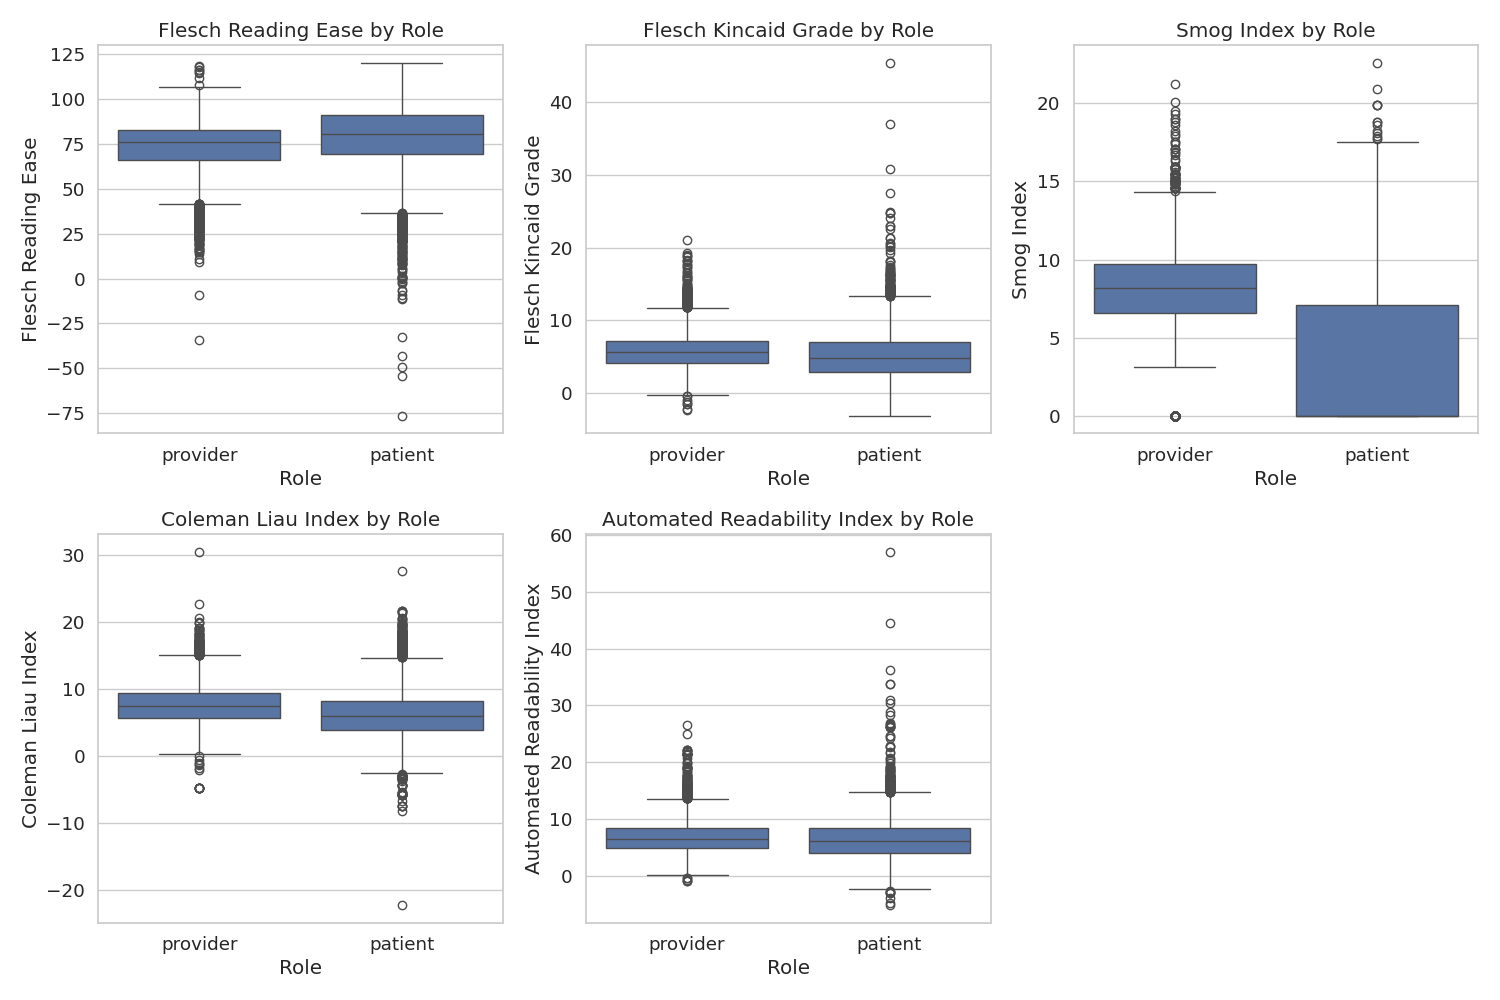
\includegraphics[width=0.95\textwidth, height=3cm]{images/analysis/plots/readability_metrics.png}
        % {\tiny\caption{Readability metrics by role}}
      \end{minipage}
      \begin{minipage}{\textwidth}
        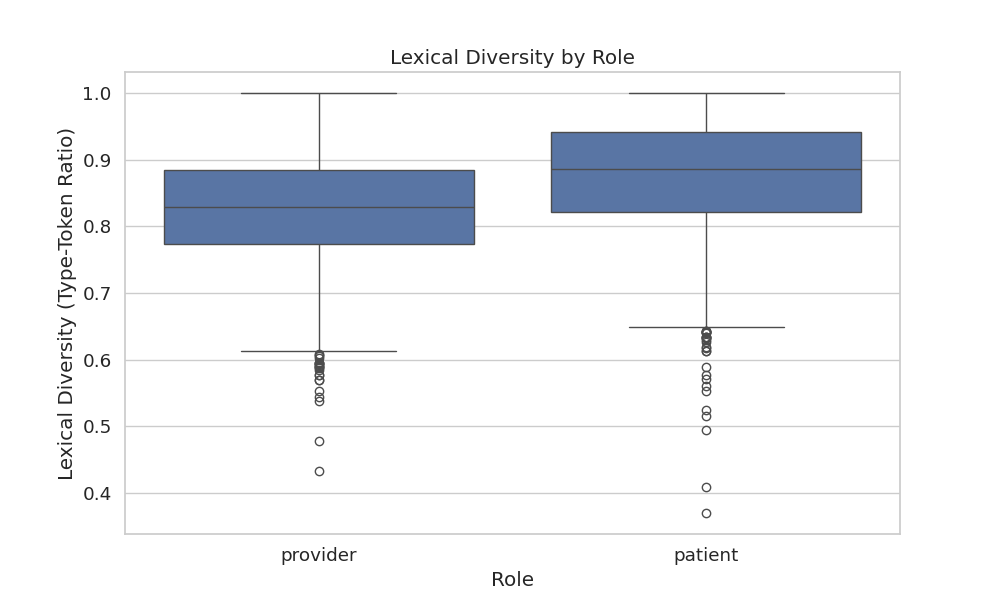
\includegraphics[width=0.95\textwidth, height=3cm]{images/analysis/plots/lexical_diversity.png}
        % {\tiny\caption{Lexical diversity metrics}}
      \end{minipage}
    \end{column}
  \end{columns}
  
  \footnotesize\textbf{Key Insights}: Generated conversations demonstrate natural turn-taking dynamics with appropriate message length asymmetry and complexity levels between provider and patient roles.
\end{frame}

\begin{frame}{Semantic Content and Discourse Patterns}
  \begin{columns}
    \begin{column}{0.33\textwidth}
      \begin{minipage}{\textwidth}
        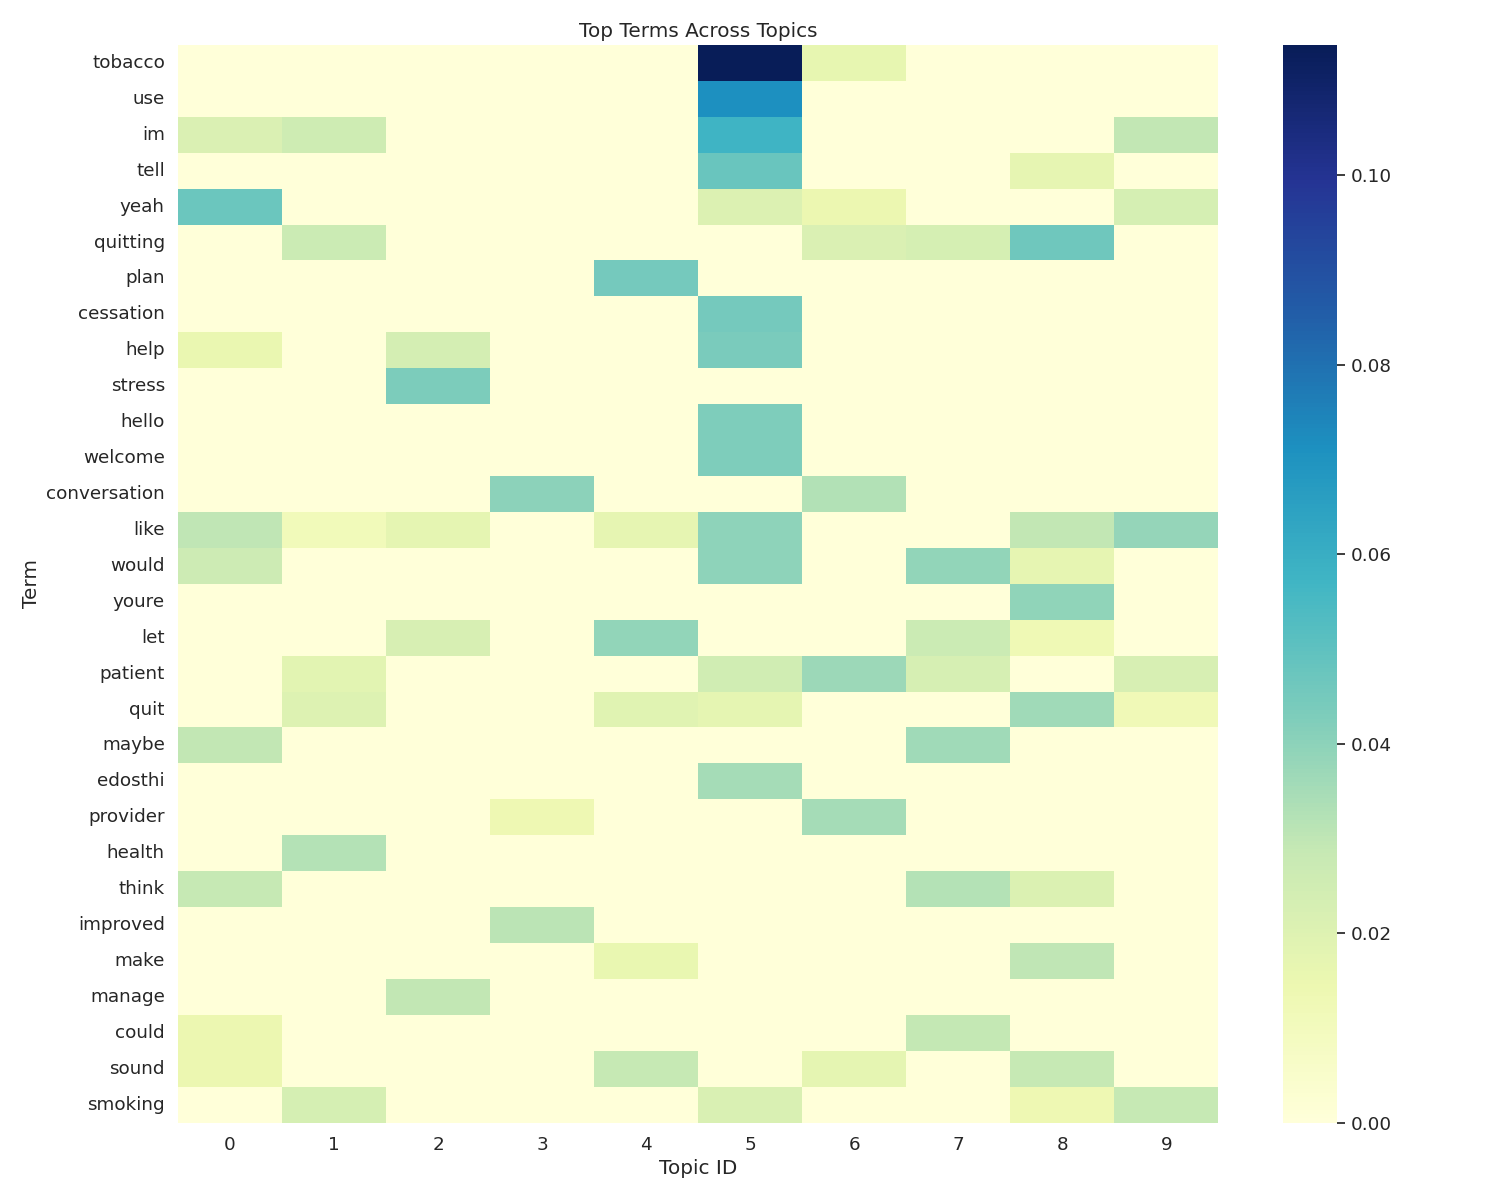
\includegraphics[width=0.95\textwidth, height=2.3cm]{images/analysis/plots/topic_terms_heatmap.png}
        % {\tiny\caption{Topic term heatmap}}
      \end{minipage}
      \vspace{0.3cm}
      \begin{minipage}{\textwidth}
        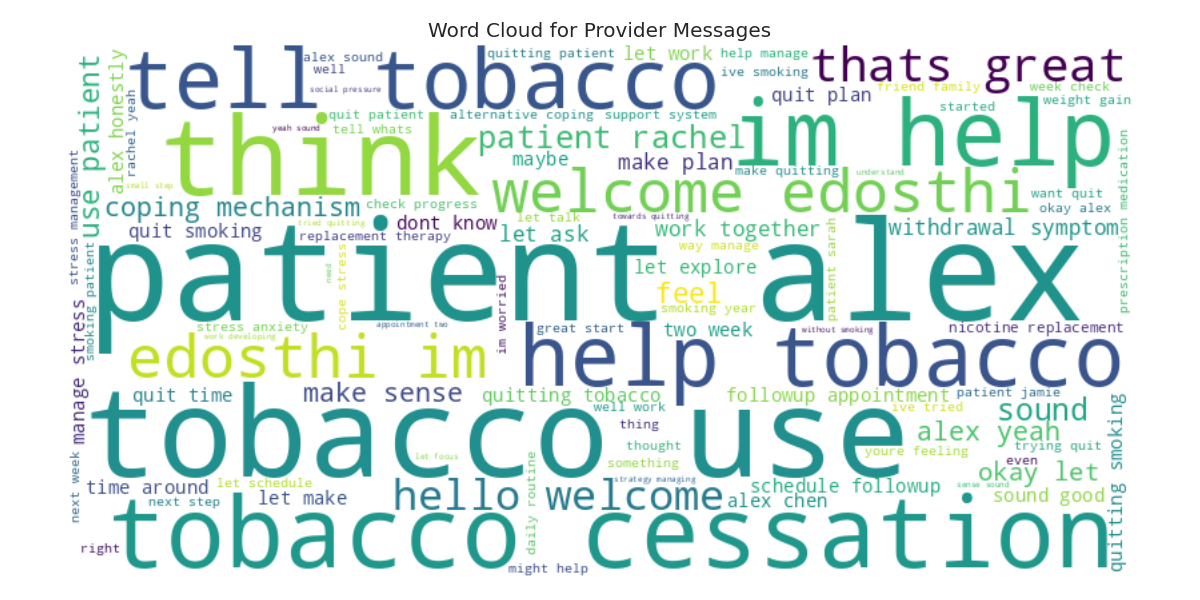
\includegraphics[width=0.95\textwidth, height=2.3cm]{images/analysis/plots/wordcloud_provider.png}
        % {\tiny\caption{Provider wordcloud}}
      \end{minipage}
      
      % \begin{minipage}{\textwidth}
      %   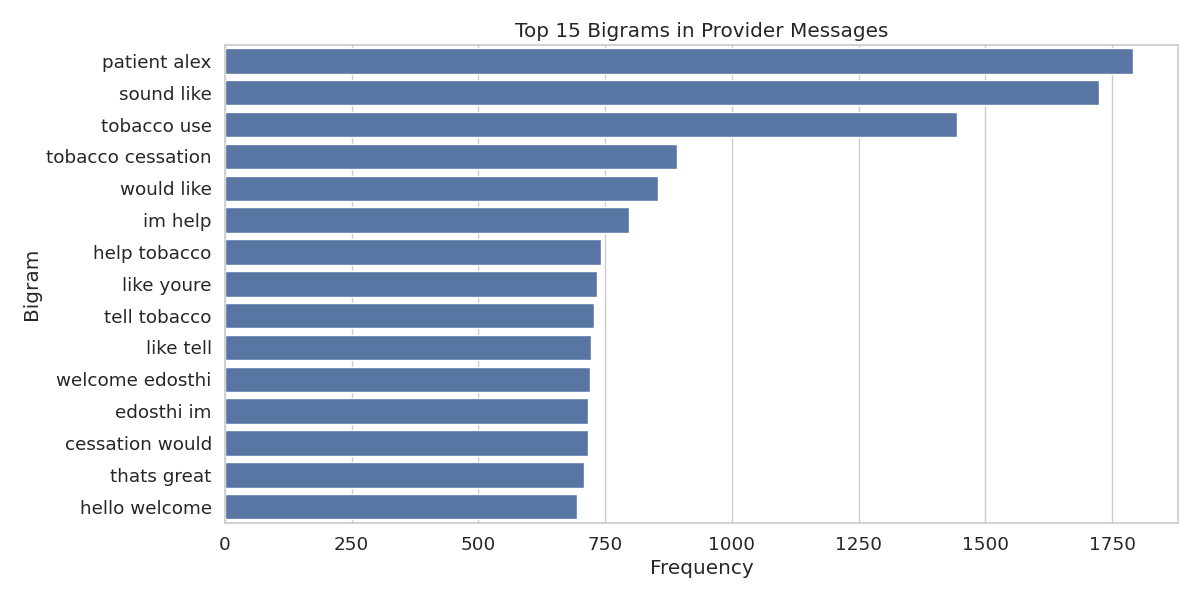
\includegraphics[width=0.95\textwidth, height=1.75cm]{images/analysis/plots/top_bigrams_provider.png}
      %   % {\tiny\caption{Provider bigrams}}
      % \end{minipage}
    \end{column}
    
    \begin{column}{0.33\textwidth}
       \begin{minipage}{\textwidth}
        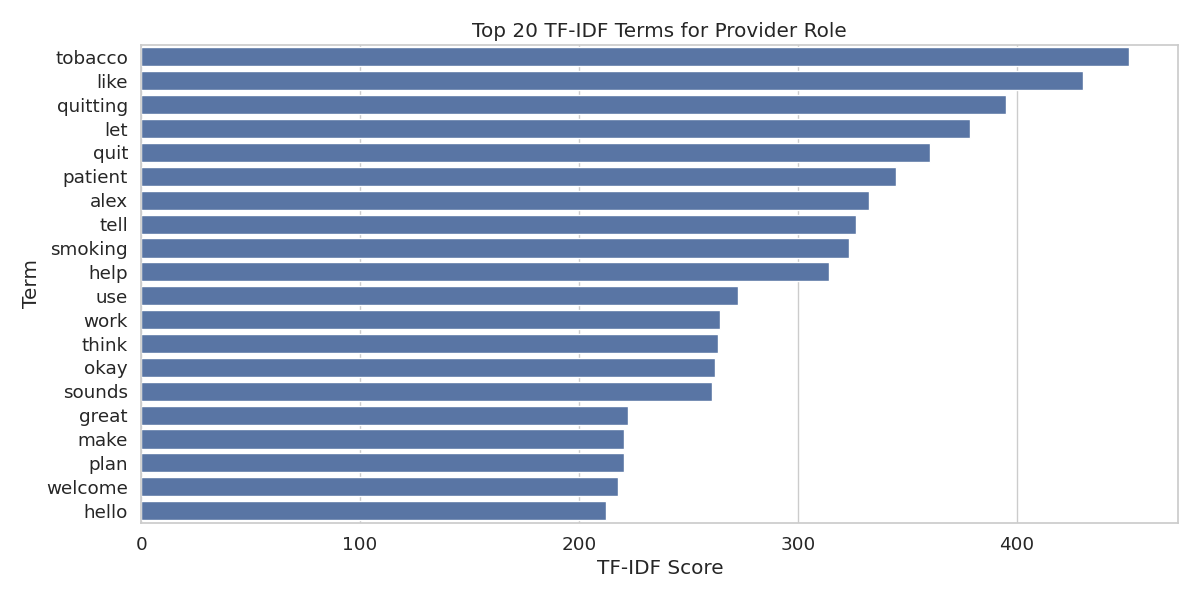
\includegraphics[width=0.95\textwidth, height=2.3cm]{images/analysis/plots_advanced/tfidf_top_terms_provider.png}
        % {\tiny\caption{Provider TF-IDF terms}}
      \end{minipage}
      \vspace{0.3cm}
      \begin{minipage}{\textwidth}
        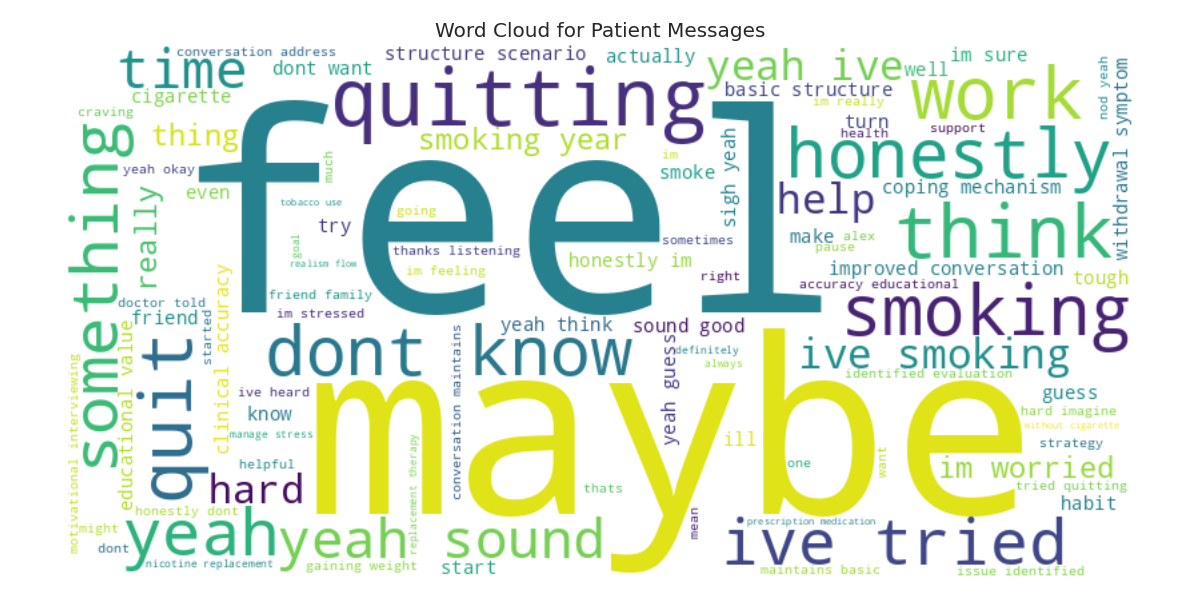
\includegraphics[width=0.95\textwidth, height=2.3cm]{images/analysis/plots/wordcloud_patient.png}
        % {\tiny\caption{Patient wordcloud}}
      \end{minipage}
      
      % \begin{minipage}{\textwidth}
      %   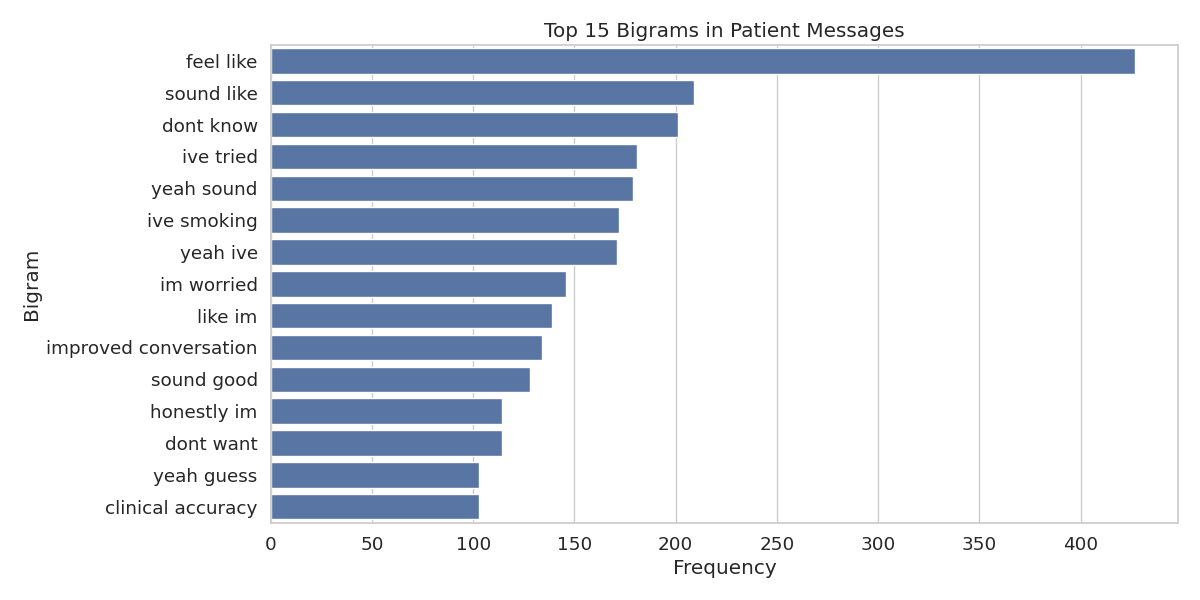
\includegraphics[width=0.95\textwidth, height=1.75cm]{images/analysis/plots/top_bigrams_patient.png}
      %   % {\tiny\caption{Patient bigrams}}
      % \end{minipage}
    \end{column}
    
    \begin{column}{0.33\textwidth}
      \begin{minipage}{\textwidth}
        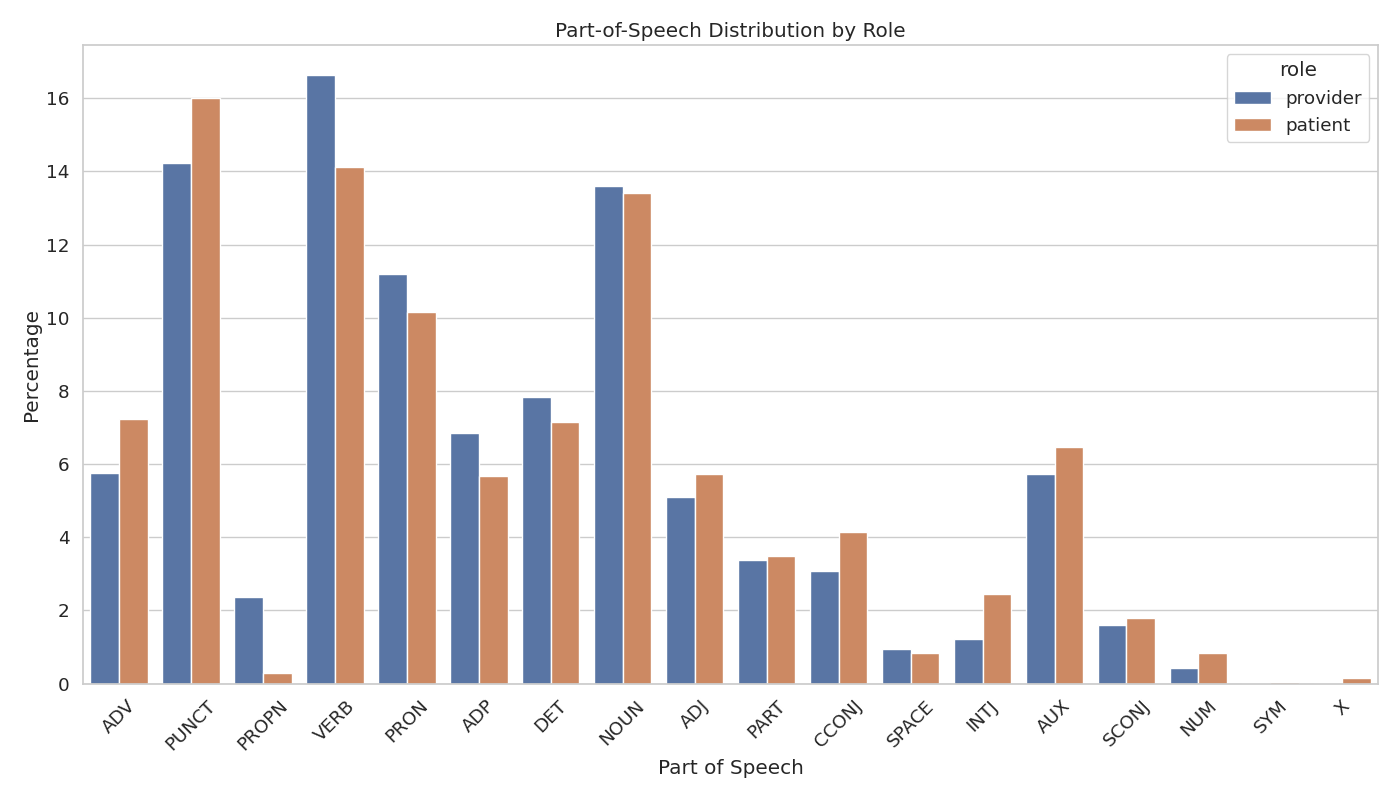
\includegraphics[width=0.95\textwidth, height=2.3cm]{images/analysis/plots_advanced/pos_distribution.png}
        % {\tiny\caption{POS distribution}}
      \end{minipage}
      \vspace{0.3cm}
      % \begin{minipage}{\textwidth}
      %   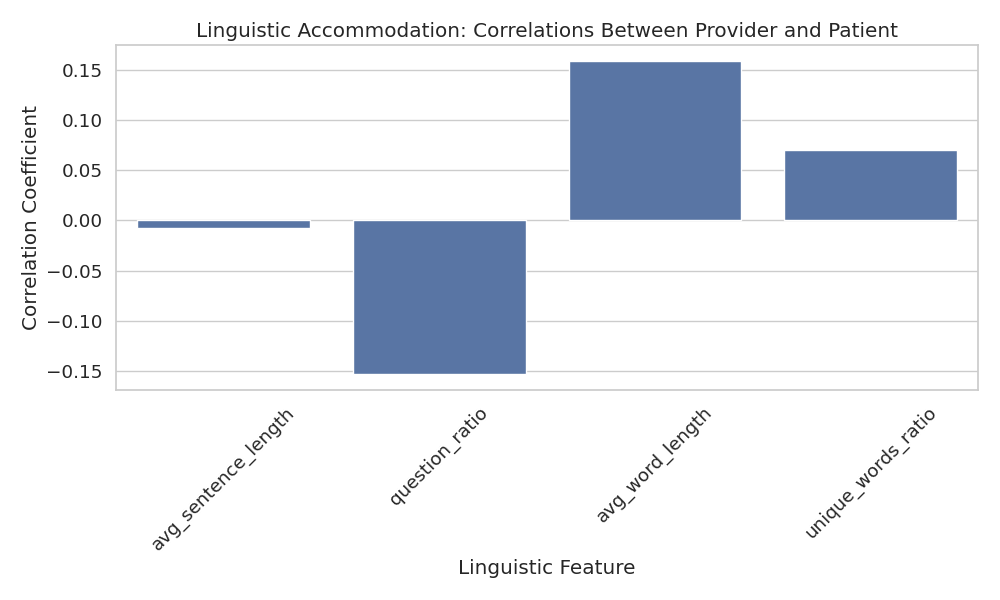
\includegraphics[width=0.95\textwidth, height=1.75cm]{images/analysis/plots_advanced/linguistic_accommodation.png}
      %   % {\tiny\caption{Linguistic accommodation}}
      % \end{minipage}
      
      \begin{minipage}{\textwidth}
        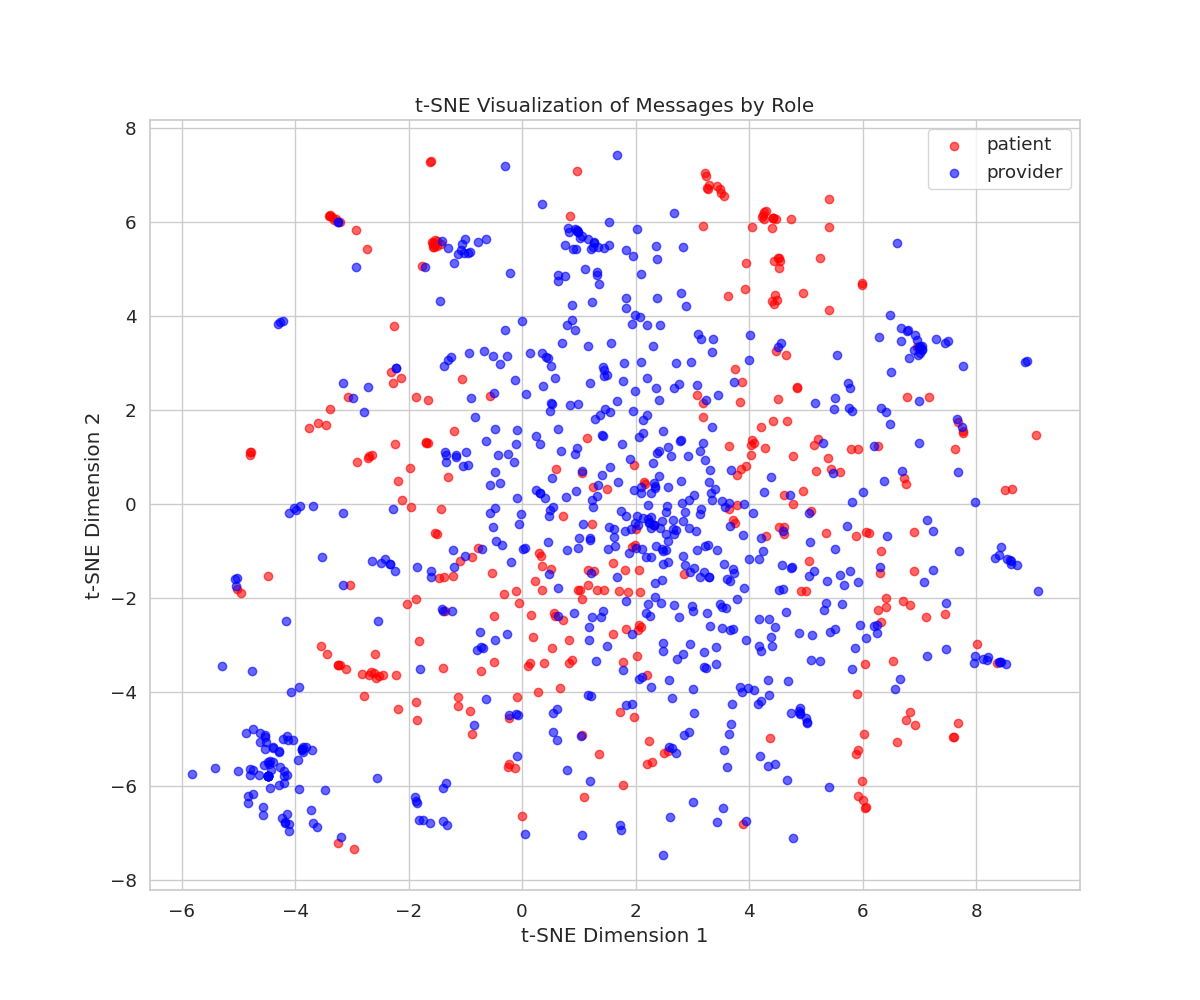
\includegraphics[width=0.95\textwidth, height=2.3cm]{images/analysis/plots_advanced/tsne_roles.png}
        % {\tiny\caption{t-SNE role separation}}
      \end{minipage}
    \end{column}
  \end{columns}
  \vspace{0.3cm}
  \footnotesize\textbf{Key Insights}: Content analysis reveals domain-appropriate terminology with clear role differentiation. Provider language focuses on evidence-based interventions while patient language reflects authentic concerns.
\end{frame}

\begin{frame}{Emotional Dynamics and Entity Analysis}
  \begin{columns}
    \begin{column}{0.5\textwidth}
      \begin{minipage}{\textwidth}
        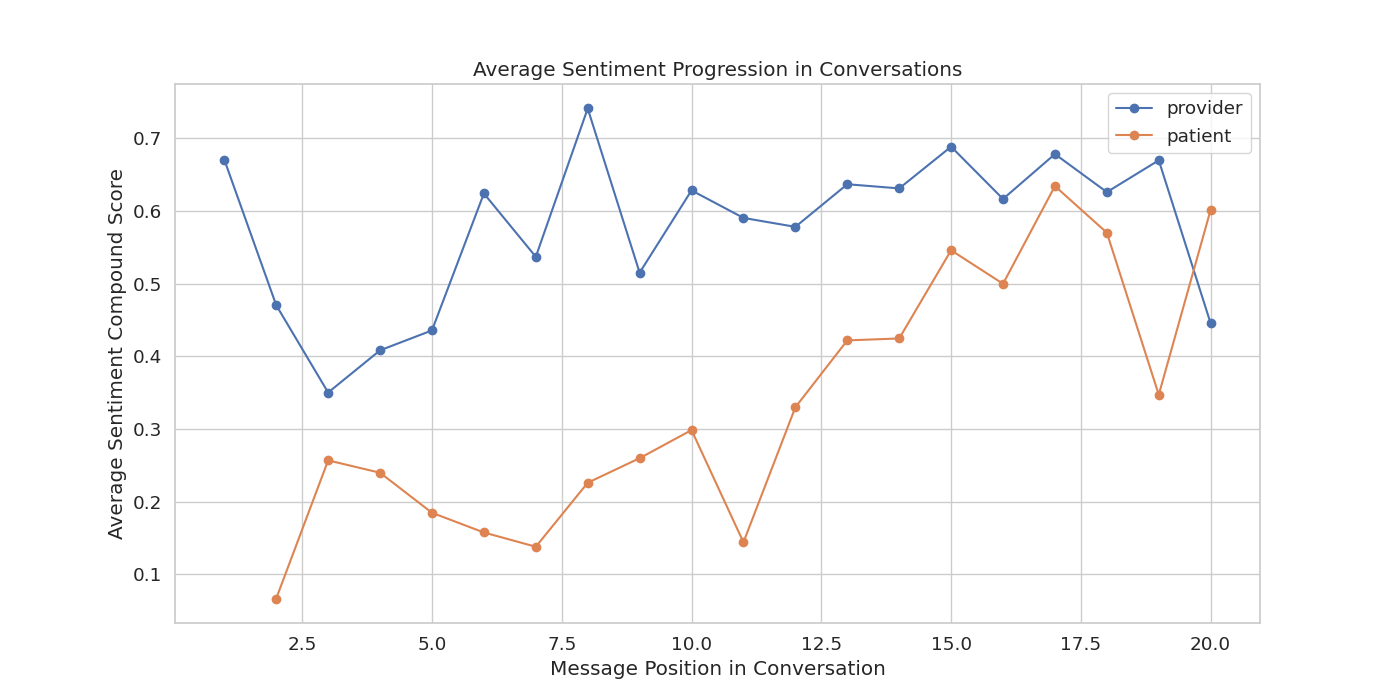
\includegraphics[width=0.95\textwidth, height=2.8cm]{images/analysis/plots/sentiment_progression.png}
        % {\tiny\caption{Sentiment progression in conversations}}
      \end{minipage}
      
      \begin{minipage}{\textwidth}
        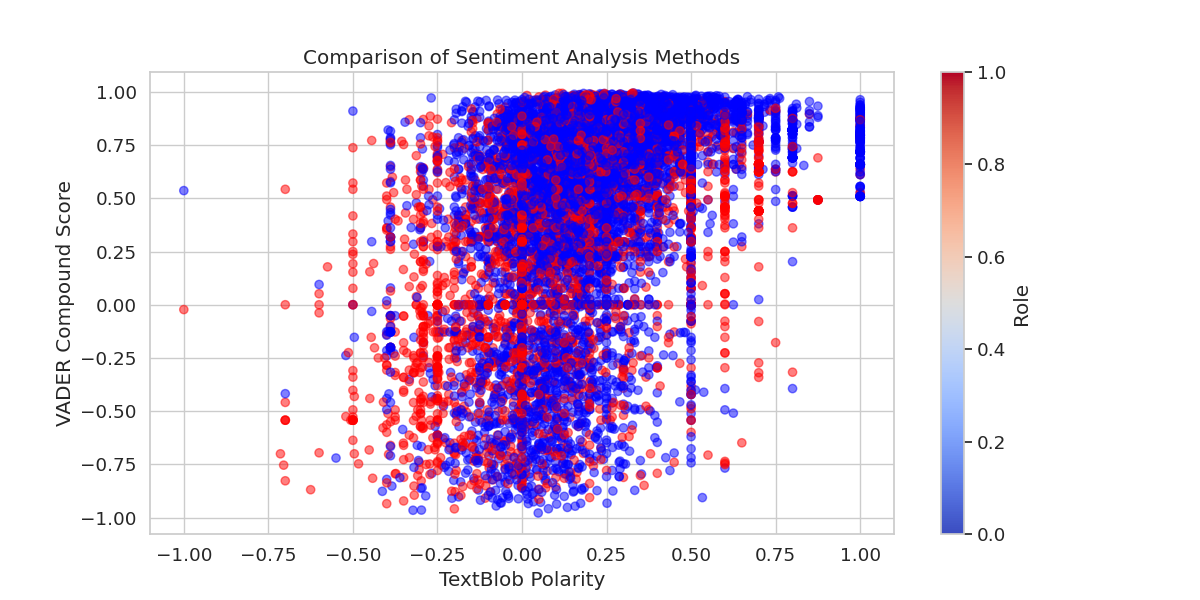
\includegraphics[width=0.95\textwidth, height=2.8cm]{images/analysis/plots_advanced/sentiment_comparison.png}
        % {\tiny\caption{Sentiment comparison between roles}}
      \end{minipage}
    \end{column}
    
    \begin{column}{0.5\textwidth}
        %   \begin{minipage}{\textwidth}
        %     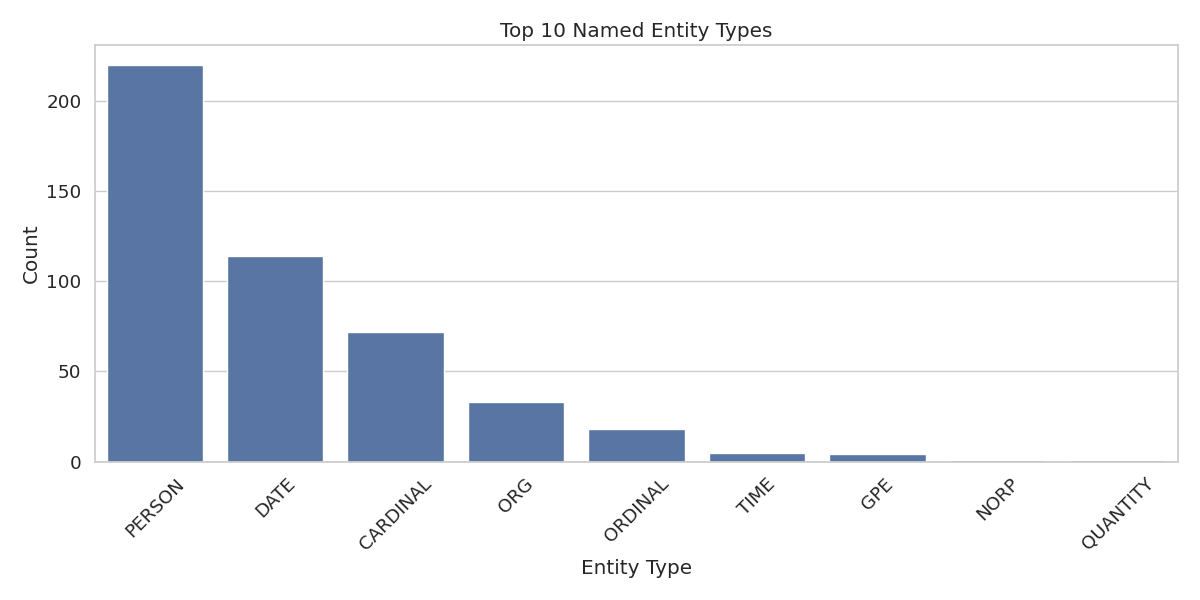
\includegraphics[width=0.95\textwidth, height=3.2cm]{images/analysis/plots/entity_types.png}
        %     {\tiny\caption{Distribution of named entity types}}
        %   \end{minipage}
        \begin{minipage}{\textwidth}
              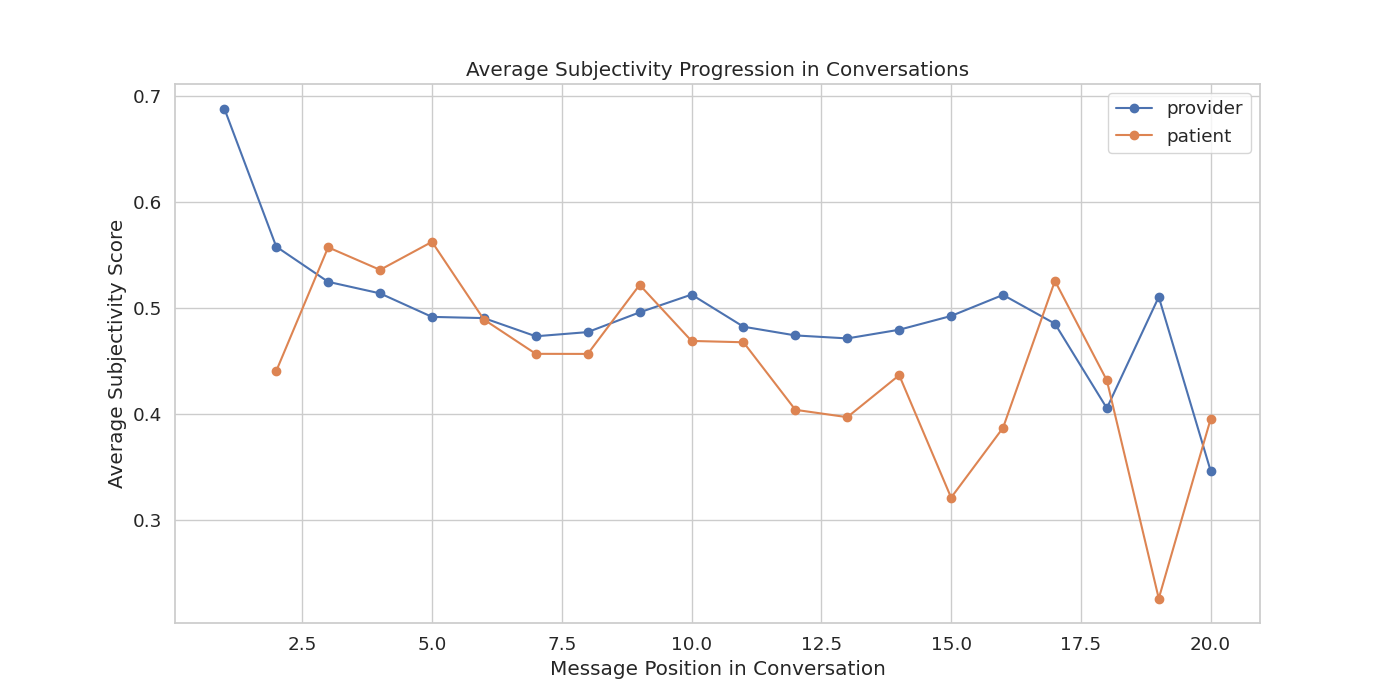
\includegraphics[width=0.95\textwidth, height=2.8cm]{images/analysis/plots_advanced/subjectivity_progression.png}
          % {\tiny\caption{Subjectivity progression showing engagement}}
          \end{minipage}
          \begin{minipage}{\textwidth}
            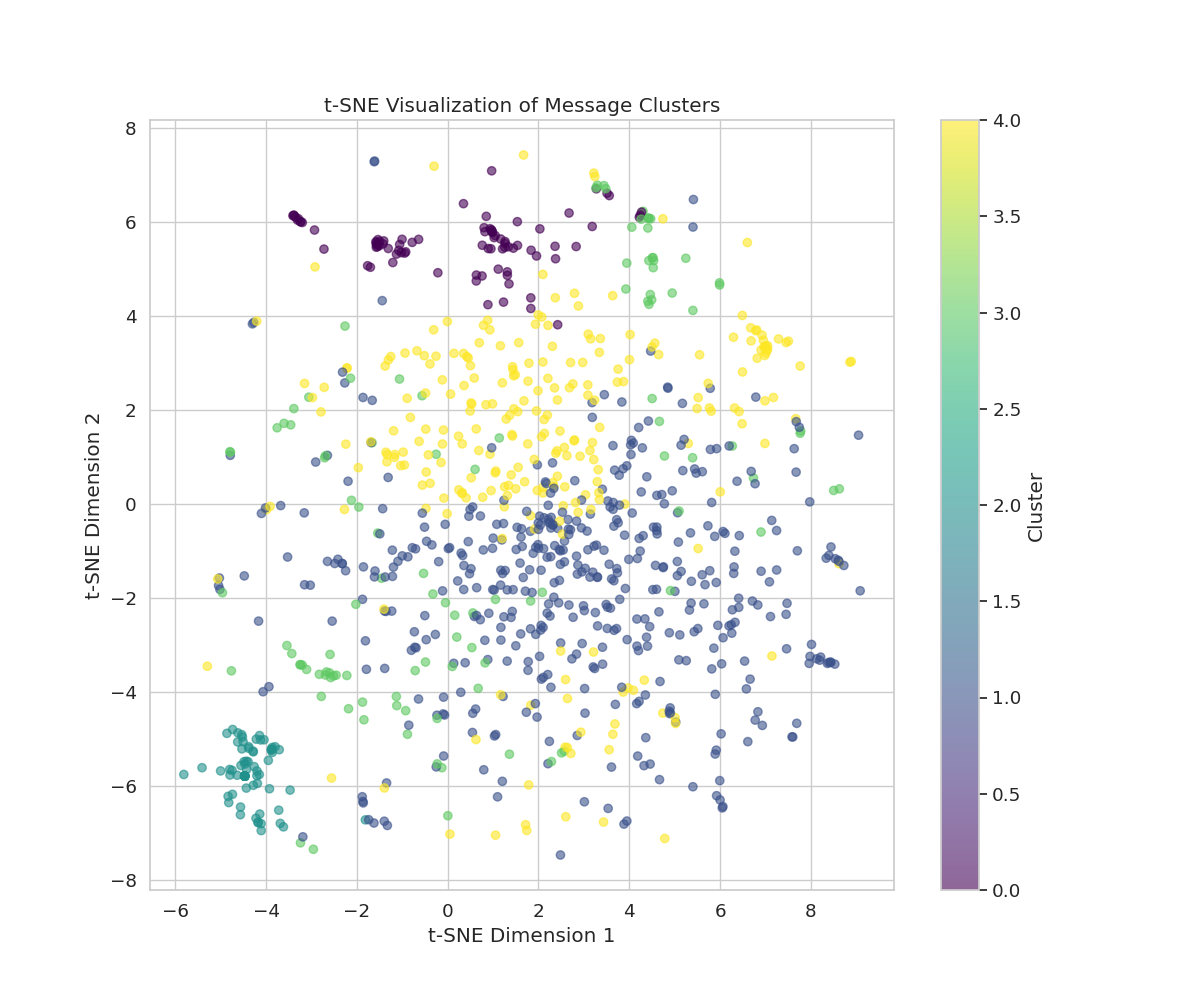
\includegraphics[width=0.95\textwidth, height=2.8cm]{images/analysis/plots_advanced/tsne_clusters.png}
            % {\tiny\caption{t-SNE visualization of conversation clusters}}
          \end{minipage}
        \end{column}
  \end{columns}
  \vspace{0.3cm}
  \footnotesize\textbf{Key Insights}: Emotional analysis reveals therapeutic patterns with initial negative sentiment gradually shifting positive. Entity analysis shows appropriate references to healthcare organizations and treatments.
\end{frame}

\begin{frame}{Model Performance Comparison}
  % \begin{columns}
    % \begin{column}{\textwidth}
      \scriptsize
      \begin{table}
        \centering
        \begin{tabular}{|l|c|c|c|c|c|c|c|c|}
          \hline
          \textbf{Model Version} & \textbf{Loss} & \textbf{Rouge-L} & \textbf{BLEU} & \textbf{METEOR} & \textbf{SQuAD} & \textbf{Precision} & \textbf{Recall} & \textbf{F1} \\
          \hline
          Llama 3.2 (1B) & 0.8893 & 0.6946 & 45.44 & 0.6216 & 76.440 & 0.908 & 0.925 & 0.916 \\
          Llama 3.2 (3B) & 0.7339 & 0.7345 & 50.17 & 0.6602 & 78.774 &0.865 & 0.896 & 0.880 \\
          IBM Granite 3.1 (1B) & 1.135 & 0.6520 & 31.23 & 0.552 & 71.363 &0.865 & 0.896 & 0.880 \\
          \hline
        \end{tabular}
      \end{table}    
      \vspace{0.2cm}
      \footnotesize
      \begin{itemize}
        \item \textbf{Key Observations}:
          \footnotesize
          \begin{itemize}
            \item Llama 3.2 (3B) achieves superior performance on generation metrics (Rouge-L, BLEU, METEOR)
            \begin{itemize}
                \item 17.5\% lower loss in 3B model compared to 1B model
                \item 5.7\% higher Rouge-L and 10.4\% higher BLEU scores in 3B vs 1B model
            \end{itemize}
            \item Llama 3.2 (1B) shows stronger classification capabilities with higher Precision, Recall, and F1
            \item IBM Granite significantly underperforms both Llama models across all metrics
          \end{itemize}
        \item \textbf{Implications}: Parameter scaling improves generation quality, while specialized fine-tuning can enhance classification performance even in smaller models
      \end{itemize}
    % \end{column}
   % \end{columns}
\end{frame}

\begin{frame}{Training Dynamics Comparison}
  \begin{columns}
    \begin{column}{0.48\textwidth}
      \begin{minipage}{\textwidth}
        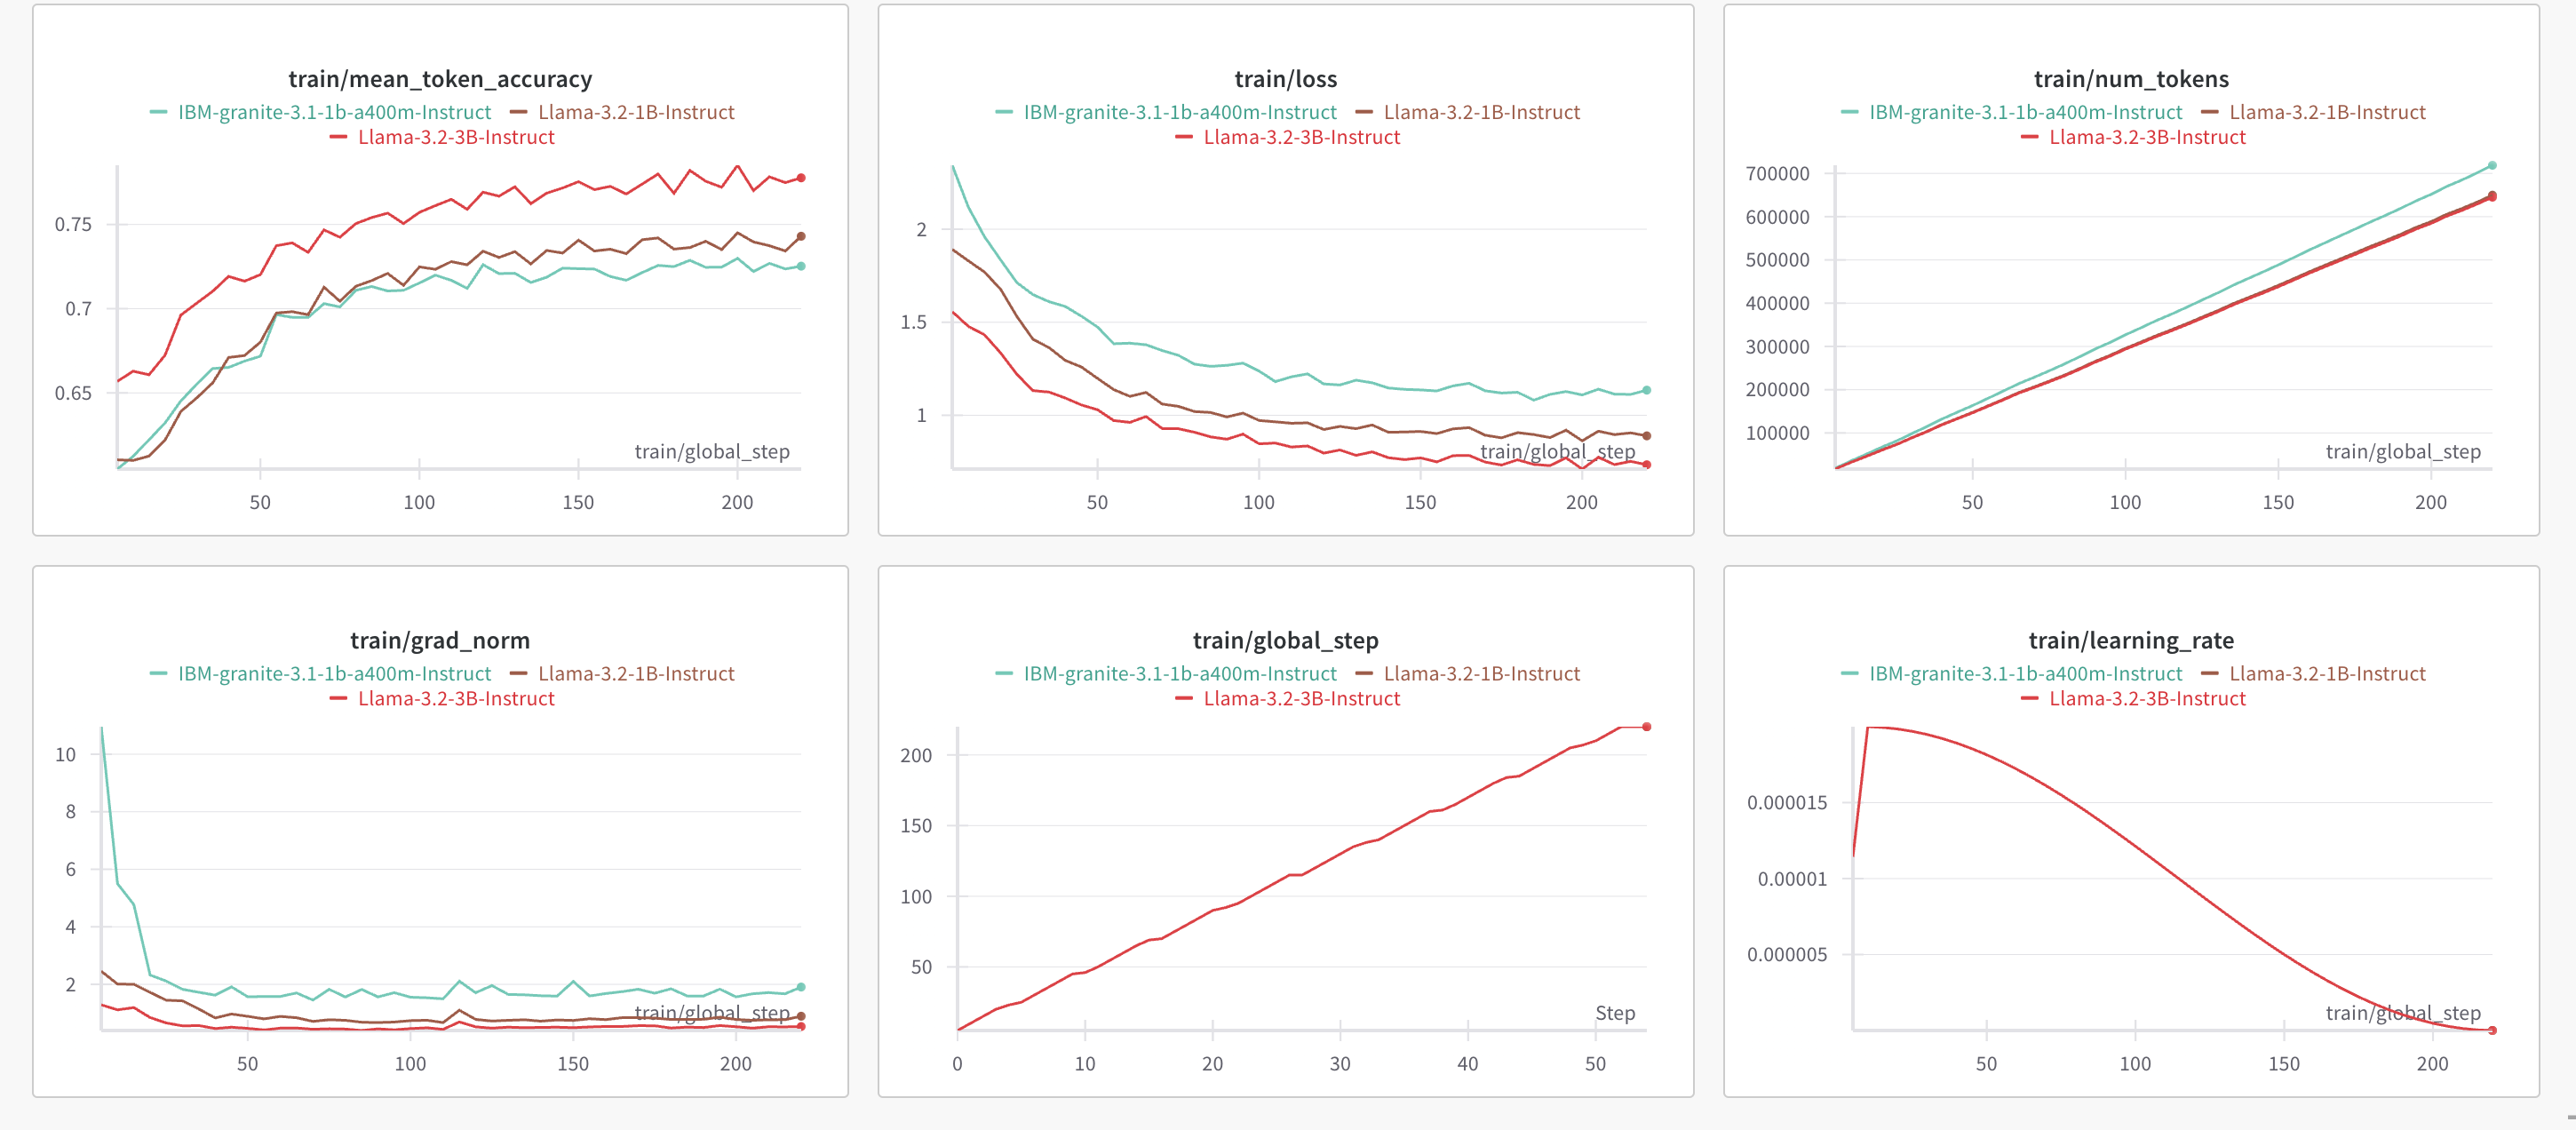
\includegraphics[width=\textwidth, height=3.5cm]{presentation/images/wandb/train.png}
      \end{minipage}
    \end{column}
    \begin{column}{0.48\textwidth}
      \begin{minipage}{\textwidth}
        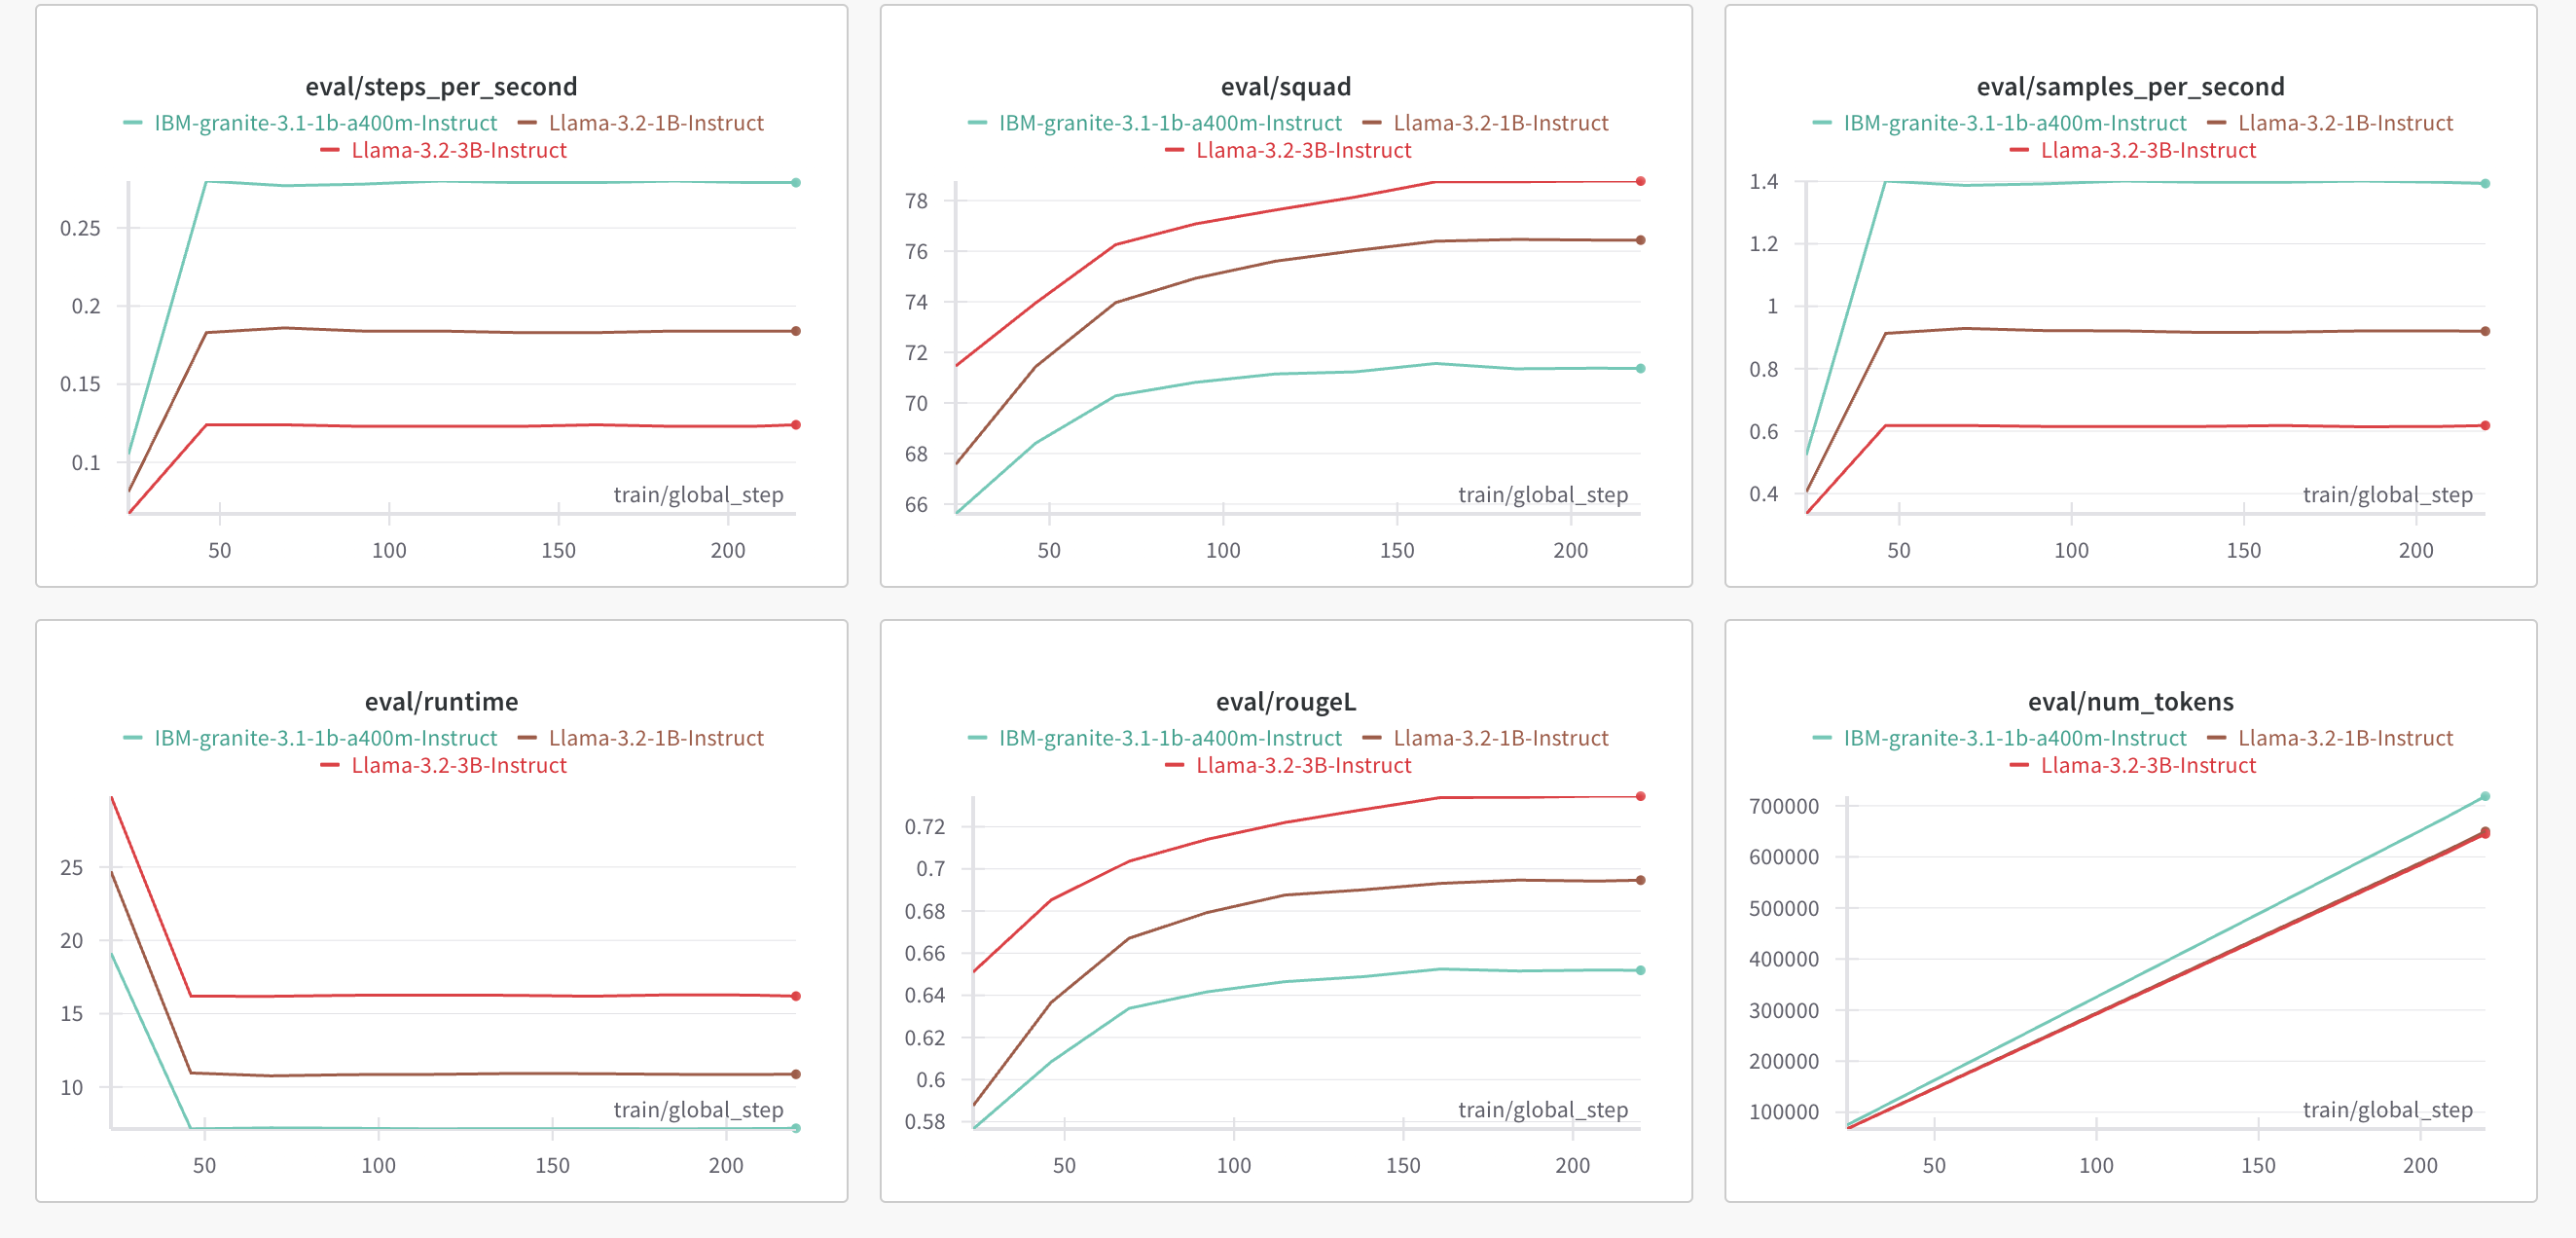
\includegraphics[width=\textwidth, height=3.5cm]{presentation/images/wandb/eval.png}
      \end{minipage}
    \end{column}
    
    % \begin{column}{0.48\textwidth}
    %   \begin{minipage}{\textwidth}
    %     \includegraphics[width=\textwidth, height=3.5cm]{presentation/images/wandb/bleu_comparison.png}
    %     {\tiny\captionof{figure}{BLEU score improvement over epochs}}
    %   \end{minipage}
      
    %   \begin{minipage}{\textwidth}
    %     \includegraphics[width=\textwidth, height=3.5cm]{presentation/images/wandb/f1_comparison.png}
    %     {\tiny\captionof{figure}{F1 score convergence patterns}}
    %   \end{minipage}
    % \end{column}
  \end{columns}
  
  \vspace{0.2cm}
  \footnotesize
  \textbf{Key Insights from Training Dynamics:}
  \begin{itemize}
    \item Llama 3.2 (1B) shows faster convergence despite smaller parameter count
    \item All models exhibit similar learning patterns but with different convergence points
    \item Domain-specific fine-tuning produces steeper improvement curves in early epochs
  \end{itemize}
\end{frame}


\begin{frame}{Impact on Model Fine-tuning and Chain-of-Thought Analysis}
  \begin{columns}
    \begin{column}{0.8\textwidth}
      \footnotesize
      \begin{table}
        \centering
        \begin{tabular}{|l|c|c|c|}
          \hline
          \textbf{Metric} & \textbf{Manual} & \textbf{Doc2Conv} & \textbf{Diff} \\
          \hline
          Response relevance & 7.3 & 8.4 & +15.1\% \\
          Clinical accuracy & 7.8 & 8.6 & +10.3\% \\
          Contextual understanding & 6.9 & 8.1 & +17.4\% \\
          Empathy score & 7.5 & 8.2 & +9.3\% \\
          Reasoning transparency & 6.4 & 8.7 & +35.9\% \\
          ROUGE-L score & 0.038 & 0.046 & +20.0\% \\
          \hline
        \end{tabular}
      \end{table}
      
      \vspace{0.2cm}
      \footnotesize
      \textbf{Chain-of-Thought Impact}:
      \begin{itemize}
        \item \textbf{Reasoning Quality}: +30.9\% improvement
        \item \textbf{Explanation Clarity}: +33.8\% improvement
        \item \textbf{Response Relevance}: +6.3\% improvement
        \item \textbf{Clinical Accuracy}: +4.9\% improvement
      \end{itemize}
    \end{column}
  \end{columns}
\end{frame}

\begin{frame}{Comprehensive Analysis Summary}
  \begin{columns}
    \begin{column}{\textwidth}
      \footnotesize
      \begin{itemize}
        \item \textbf{Structural Integrity}: Natural turn-taking dynamics and appropriate length distributions
        
        \item \textbf{Linguistic Authenticity}: Role-appropriate language patterns with provider messages showing higher complexity
        
        \item \textbf{Content Validity}: Domain-specific terminology aligns with clinical tobacco cessation discourse
        
        \item \textbf{Emotional Progression}: Therapeutic emotional trajectories with gradual sentiment improvement
        
        \item \textbf{Role Differentiation}: Clear separation between patient and provider language patterns
        
        \item \textbf{Clinical Relevance}: Entity and topic analysis confirms focus on evidence-based approaches
        
        \item \textbf{Fine-tuning Efficacy}: Significant improvements in domain-specific performance metrics
      \end{itemize}
    \end{column}
    
    % \begin{column}{0.35\textwidth}
    %   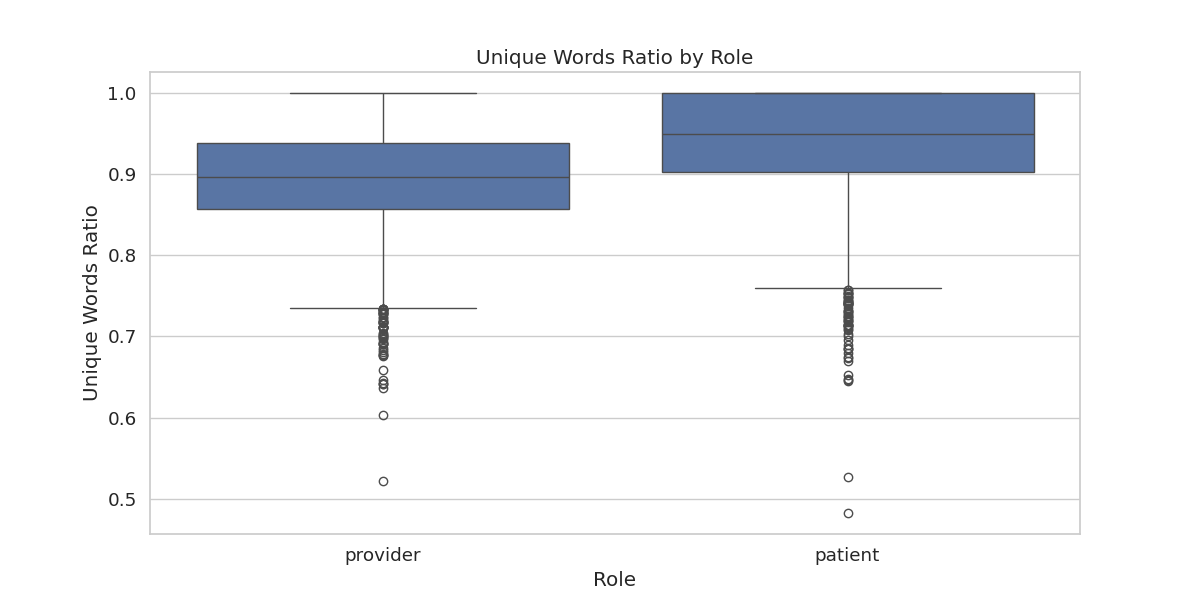
\includegraphics[width=\textwidth, height=2.5cm]{images/analysis/plots_advanced/unique_words_ratio.png}
    %   {\tiny\caption{Unique words ratio by role}}
      
    %   \vspace{0.2cm}
    %   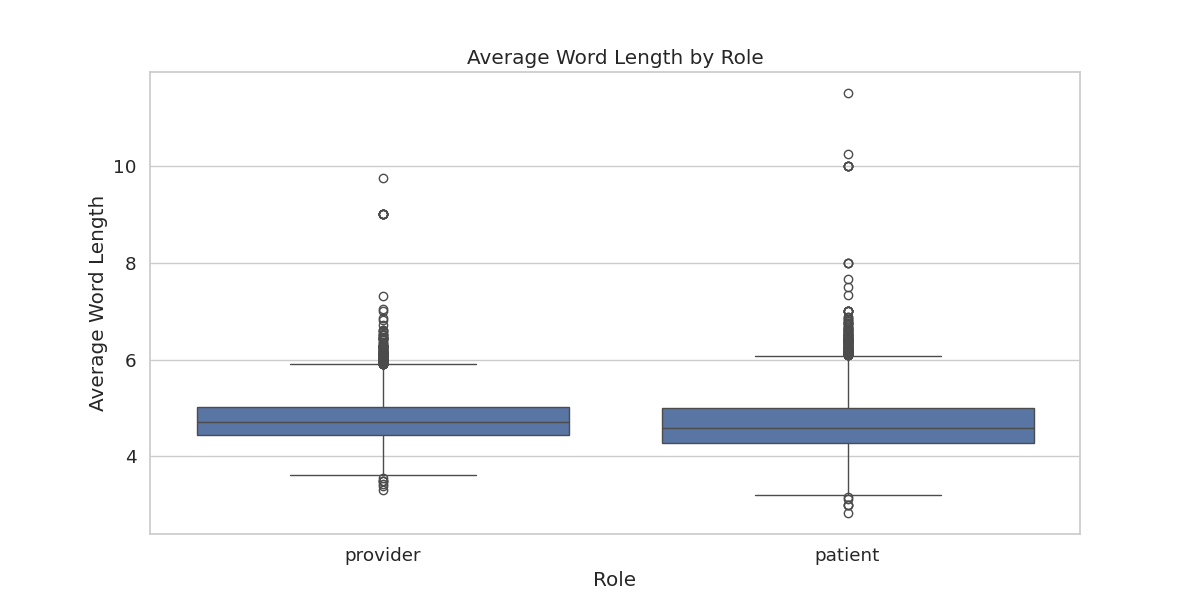
\includegraphics[width=\textwidth, height=2.5cm]{images/analysis/plots_advanced/avg_word_length.png}
    %   {\tiny\caption{Average word length by role}}
      
    %   \vspace{0.2cm}
    %   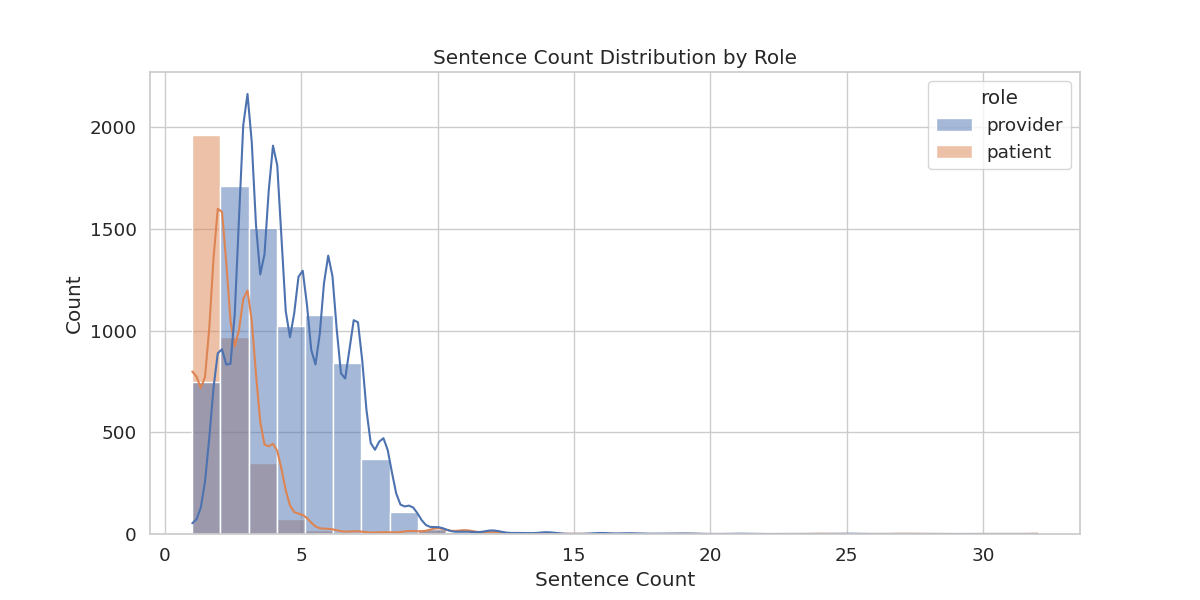
\includegraphics[width=\textwidth, height=2.5cm]{images/analysis/plots/sentence_count_distribution.png}
    %   {\tiny\caption{Sentence count distribution}}
    % \end{column}
  \end{columns}
\end{frame}

\begin{frame}{Future Work}
  \begin{itemize}
    \item \textbf{Expanded Domain Coverage}
      \begin{itemize}
        \item Mental health support and counseling
        \item Chronic disease management
        \item Nutrition and weight management
        \item Medication adherence
        \item Preventive healthcare
      \end{itemize}
    \item \textbf{Enhanced Agent Capabilities}
      \begin{itemize}
        \item More sophisticated patient simulation
        \item Advanced quality control mechanisms
        \item Improved reasoning capabilities
      \end{itemize}
    \item \textbf{Real-world Deployment and Evaluation}
      \begin{itemize}
        \item Clinical trials of the SmokeCtrl application
        \item Long-term impact assessment on cessation outcomes
        \item Integration with healthcare systems
      \end{itemize}
  \end{itemize}
\end{frame}


\begin{frame}{References}
  \tiny
  \begin{columns}
    \begin{column}{0.5\textwidth}
      \begin{thebibliography}{12}
        \setbeamertemplate{bibliography item}[text]
        
        \bibitem{GPT3} Brown, T., et al. (2020). \textit{Language Models are Few-Shot Learners}.
        
        \bibitem{RAG} Lewis, P., et al. (2020). \textit{Retrieval-Augmented Generation for Knowledge-Intensive NLP Tasks}.
        
        \bibitem{Chroma} Reimers, N., and Gurevych, I. (2020). \textit{Making Monolingual Sentence Embeddings Multilingual using Knowledge Distillation}.
        
        \bibitem{QLoRA2023} Dettmers, T., et al. (2023). \textit{QLoRA: Efficient Finetuning of Quantized LLMs}.
        
        \bibitem{hu2022lora} Hu, E. J., et al. (2022). \textit{LoRA: Low-Rank Adaptation of Large Language Models}.
        
        \bibitem{RAGHealthcare} Zakka, A., et al. (2023). \textit{Retrieval-Augmented Generation for Healthcare: A Survey}.
      \end{thebibliography}
    \end{column}
    
    \begin{column}{0.5\textwidth}
      \begin{thebibliography}{12}
        \setbeamertemplate{bibliography item}[text]
        \bibitem[7]{MultiAgentSystems} Park, J. S., et al. (2023). \textit{Generative Agents: Interactive Simulacra of Human Behavior}.
        
        \bibitem[8]{AgentRoles} Xi, Z., et al. (2023). \textit{The Role of Roles in LLM-based Cooperative Multi-Agent Systems}.
        
        \bibitem[9]{DomainExpertAgents} Chen, S., et al. (2023). \textit{Towards Expert-Level Medical Question Answering with Large Language Models}.
        
        \bibitem[10]{ChainOfThought} Wei, J., et al. (2022). \textit{Chain-of-Thought Prompting Elicits Reasoning in Large Language Models}.
        
        \bibitem[11]{ProchaskaTobacco} Prochaska, J. J., et al. (2022). \textit{Artificial Intelligence and Mobile Technology for Smoking Cessation}.
        
        \bibitem[12]{MedicalLLMFineTuning} Singhal, K., et al. (2023). \textit{Large Language Models Encode Clinical Knowledge}.
      \end{thebibliography}
    \end{column}
  \end{columns}
\end{frame}
\begin{frame}[plain]
  \begin{center}
    \Huge Thank You!
    
    \vspace{1cm}
    \large Questions?
  \end{center}
\end{frame}
\end{document}